\documentclass[a4paper,12pt]{article}

% Packages
\usepackage{hyperref}
\hypersetup{
    colorlinks=true,
    linkcolor=black,     % Internal links (like Table of Contents)
    citecolor=blue,      % Citations
    urlcolor=cyan        % External URLs
}
\usepackage{graphicx}
\usepackage{amsmath}
\usepackage{geometry}
\usepackage{fancyhdr}
\usepackage{setspace}
\usepackage{booktabs}
\usepackage{titlesec}  % For title formatting
\geometry{margin=1in}
\setstretch{1.5}
\usepackage{listings}
%font greek
\usepackage[utf8]{inputenc}
\usepackage[greek,english]{babel}
\usepackage{alphabeta}
% Header and Footer
\pagestyle{fancy}
\fancyhf{}
\fancyhead[R]{\thepage}
\usepackage{minted}
\usepackage[round]{natbib} % For (Devlin et al., 2019)

%Coding
\usepackage{xcolor,listings}
\usepackage{textcomp}
\lstset{upquote=true}
\usepackage{courier} %% Sets font for listing as Courier.
\lstset{
showstringspaces = false, %% prevent space marking in strings, string is defined as the text that is generally printed directly to the console
numbers = left, %% display line numbers on the left
commentstyle = \color{green}, %% set comment color
keywordstyle = \color{blue}, %% set keyword color
stringstyle = \color{black}, %% set string color
rulecolor = \color{black}, %% set frame color to avoid being affected by text color
basicstyle = \small \ttfamily , %% set listing font and size
breaklines = true, %% enable line breaking
numberstyle = \tiny,
}

% Title Formatting
\titleformat{\section}{\normalfont\Large\bfseries}{\thesection}{1em}{}

\setcounter{secnumdepth}{3}
\setcounter{tocdepth}{3}

\begin{document}
\begin{titlepage}
    \begin{center}
        \LARGE
        \textbf{Theoretical Project }\\
        \large
        \textbf{Data Mining \& Learning Algorithms}

        \vspace{1cm}
        
\includegraphics[width=5cm]{img/upatras.jpg}
        \vspace{1cm}

        {\large \textbf{Team Composition}}\\
        Νικόλαος Δερεκενάρης (1100529) \\ 4th Year,
        up1100529@ac.upatras.gr, \\
        \vspace{0.25cm}
        Μητρογιάννης Ευάγγελος (1100626) \\ 4th Year,
        up1100626@ac.upatras.gr, \\
        \vspace{6cm}


        Computer Engineering \& Informatics Department\
        University of Patras \\
        Spring Semester 2025-26
    \end{center}
\end{titlepage}

\newpage

\tableofcontents


\clearpage
\section{Introduction}
This report focuses on the study of the Bert Transformer architecture for deep language understanding. After a short description of the state of NLP around the time when Transformers came along and revolutionized the field, we will continue with a brief overview behind the novel idea of the original Transformer that led to it's inception \citep{vaswani2017attention} and then summarize the original paper \citep{devlin2019bert} and its influence. 

To facilitate the main objective of this report, we will further our focus on a number of \textit{State-Of-The-Art} (SOTA) implementations utilizing the BERT Transformer, their different approaches, and philosophies, as well as expand this study even further, by focusing on some more foundational papers that have been published in the last few years, which have been inspired by the original BERT paper and or the transformer architecture in general.

\section{The State of NLP in 2017}
Prior to the introduction of the Transformer architecture, the prevailing paradigm in NLP relied almost exclusively on seq2seq models rooted in Recurrent Neural Networks (RNNs). While architectures such as LSTMs \citep{hochreiter1997long} and GRUs were designed to mitigate the vanishing gradient problem, several fundamental bottlenecks persisted.

\subsection{Sequential Processing and Parallelization}
The defining characteristic of RNNs is their sequential nature; they process tokens one by one, maintaining a hidden state $h_t$ that is dependent on the previous state $h_{t-1}$. This linear dependency creates a significant computational bottleneck, as it prevents parallelization during training. As datasets grew in the mid-2010s, the inability to leverage GPU hardware to its full extent became a primary constraint on model scaling.

\subsection{The Long-Range Dependency Problem}
Despite the memory gates in LSTMs, these models struggled to capture dependencies between words that were far apart in a sentence. The signal of a word at the beginning of a long sequence often became diluted by the time the model reached the end. This was largely a consequence of the \textit{representation bottleneck}, where the model attempted to compress the semantic information of an entire variable-length input sequence into a single fixed-length context vector. While early attention mechanisms \citep{bahdanau2014neural} were introduced to allow the decoder to "look back" at specific encoder states, they were still auxiliary components added onto an underlying recurrent structure.

\subsection{Static vs. Contextual Embeddings}
In 2017, the industry standard for word representation involved static embeddings such as Word2Vec or GloVe. These methods assigned a single fixed vector to each word (e.g., the word "bank" would have the same vector regardless of whether the context was financial or geographical). While contemporaneous models like ELMo began experimenting with context-sensitive representations using Bi-LSTMs, the field was ripe for a non-recurrent architecture that could process entire sequences bi-directionally and simultaneously.

This vacuum set the stage for the "Attention is All You Need" paper, which proposed a radical departure: discarding recurrence entirely in favor of the Self-Attention mechanism.

\section{The Transformer Revolution}
In 2017, \cite{vaswani2017attention} published "Attention Is All You Need", proposing an architecture that discarded recurrence and convolution entirely in favor of a mechanism known as \textit{Self-Attention}. This shift allowed for unprecedented parallelization and solved the long-range dependency issues that had plagued the field.

\subsection{The Core Architecture}
The original Transformer was built to solve Machine Translation. That is, for a given text sequence as input, for example in French (\textit{Je suis etudiant}), for the model to output its English translation (\textit{I am a student}), or any other language for that matter. Its architecture consisted of two parts. An encoder stack and a decoder stack.

\begin{figure}[H]
    \centering
    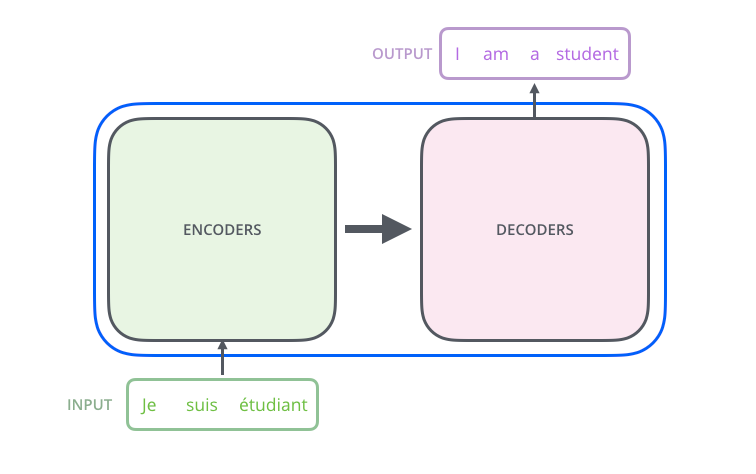
\includegraphics[width=0.75\linewidth]{img/transformer_architecture_high.png}
    \caption{High level view of the Transformer architecture}
    \label{fig:placeholder}
\end{figure}
 
In the original paper, the encoder stack consisted of six identical encoders, stacked on top of each other. It should be noted that there is nothing inherently special about the number six, any different number of arrangements is possible. The decoder stack also stacks six decoders on top of each other.

\begin{figure}[H]
    \centering
    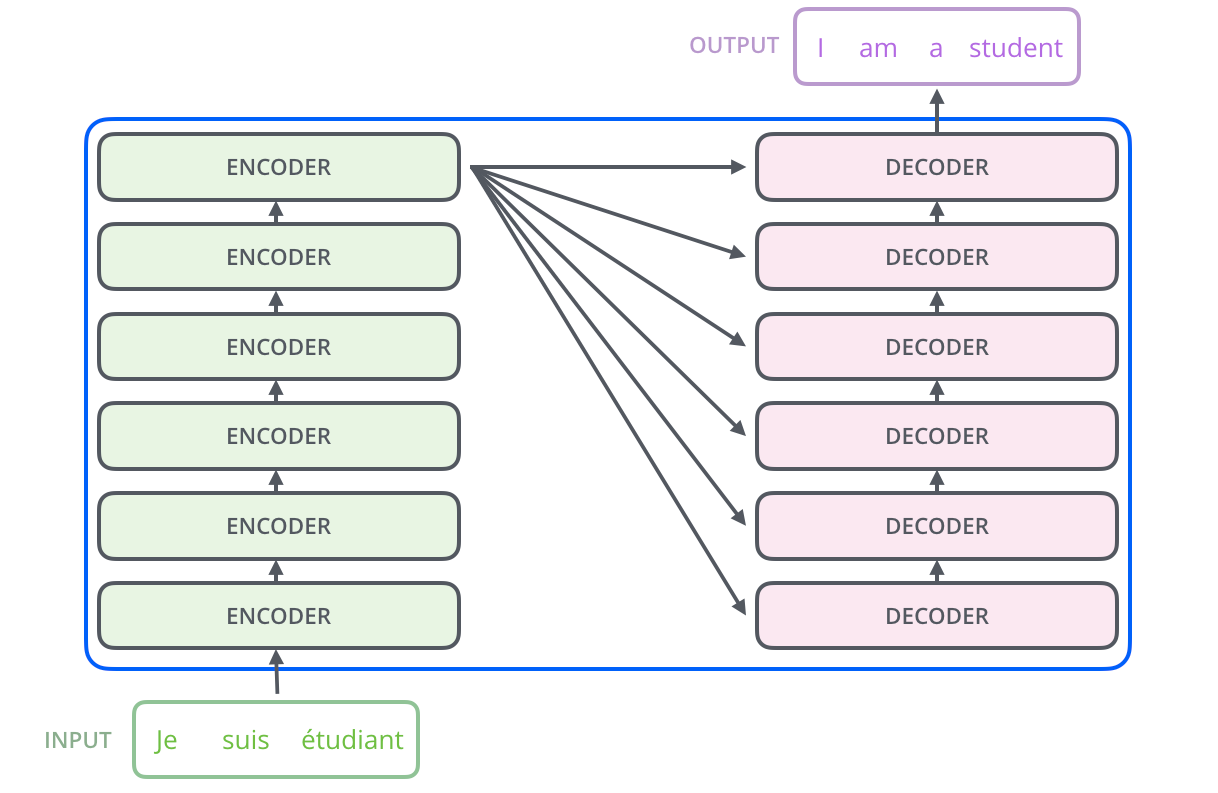
\includegraphics[width=0.75\linewidth]{img/xray_encoder.png}
    \caption{Inter structure of Encoder and Decoder modules}
    \label{fig:placeholder}
\end{figure}

The encoders are all identical in structure. They consist of two layers. The first layer is the so called \textit{Self-Attention} layer, and the second layer is a simple feed forward network. Both layers are wrapped in a residual connection and followed by layer normalization.

The decoder modules are also identical in structure, and they consist of three layers. The first layer is a masked self-attention layer, the second layer is a regular attention layer that attends to the output of the encoder stack, and the third layer is a feed forward network. Similar to the encoder, all three layers are wrapped in residual connections and followed by layer normalization.

\begin{figure}[H]
    \centering
    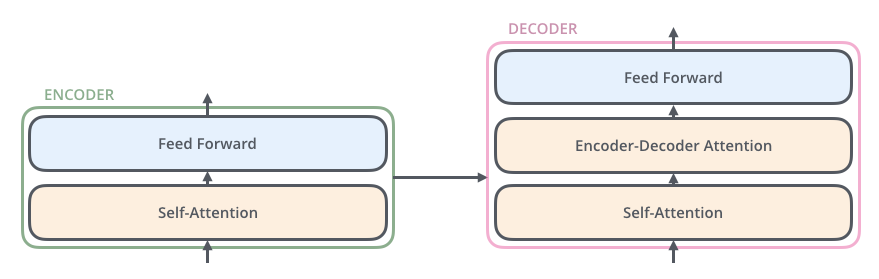
\includegraphics[width=0.75\linewidth]{img/enc_dec_layers.png}
    \caption{Module Internal Structure}
    \label{fig:placeholder}
\end{figure}

\subsubsection{Self-Attention}
The self-attention mechanism is at the core of the transformer and the main reason for its success. Past architectures had to rely on recurrence to capture the dependencies between tokens in a sequence. The self-attention mechanism allows the model to directly attend to all positions in the input sequence simultaneously, regardless of their distance from each other. This is achieved by computing attention weights that determine how much each token should attend to every other token in the sequence when generating its representation.

The \textbf{first step} in calculating self-attention is to create three vectors from each of the encoder's input vectors, which at the beginning step are just the static embedding of each word (positional encodings are also added to the input embeddings to inject information about the position of each token in the sequence). These three vectors are the Query ($Q$), Key ($K$), and Value ($V$) vectors. Each of these is obtained by multiplying the input embedding by a learned weight matrix ($W^Q$, $W^K$, $W^V$). 

The \textbf{second step} is to compute a score for each token in the sequence. Let's imagine the input sentence "Blue Cheese" and let's assume it consists of the tokens "Blue" and "Cheese". When calculating the self-attention score for the token "Blue", we need to score each other token in the sequence against this token. The score determines how much attention the current token should pay to the rest of the tokens in the sequence, in order to create its representation. 

The score is computed by taking the dot product of the target token's query vector against the key vector of the token we are scoring against. In our example, to calculate the score of "Blue", we would take the dot product of the query vector of "Blue" first against itself, and then against the token "Cheese". That is, $q_1 \cdot k_1$, and $q_1 \cdot k_2$ respectively. 

The \textbf{third step} is to scale the scores by $\frac{1}{\sqrt{d_k}}$, where $d_k$ is the dimension of the keys. This scaling step is a critical "safety valve" for gradients. Without it, for large values of $d_k$, the dot products could grow extremely large in magnitude, pushing the softmax function into regions where its gradient is extremely small, leading to the vanishing gradient problem during backpropagation.

The \textbf{fourth step} is to  apply a softmax function to obtain the attention weights. In the above example, if $\frac{q_1 \cdot k_1}{\sqrt{d_k}}=112$, and $\frac{q_1 \cdot k_2}{\sqrt{d_k}}=96$, the softmax would give the scores $0.88$ and $0.12$ respectively. This means that the token "Blue" would attend to itself with a weight of $0.88$ and to "Cheese" with a weight of $0.12$. 

The \textbf{fifth step} is to multiply each token's value vector by the corresponding softmax score and then sum the weighted value vectors to obtain the output of the self-attention layer for the target token. In our example, the output for "Blue" would be $0.88 \cdot v_1 + 0.12 \cdot v_2$.

In the actual implementation, the above happen in matrix form, so we'll shortly describe that as well. 

\textbf{First,} we pack all of our input embeddings into one matrix $X$, and then take the dot product of $X$ with $W^Q$, $W^K$, and $W^V$ to obtain the $Q$, $K$, and $V$ matrices respectively. So, $Q = XW^Q$, $K = XW^K$, and $V = XW^V$. 

Finally, steps two to five can be described as follows:
\begin{equation}
    Z = \text{softmax}\left(\frac{QK^T}{\sqrt{d_k}}\right)V
\end{equation}
Where $Z$ is the output of the self-attention layer. Each row of $Z$ corresponds to the new representation of each token in the input sequence, which is a weighted sum of the value vectors of all tokens, where the weights are determined by the attention scores.

\subsubsection{Multi-Headed Attention}
The process described above is called "Scaled Dot-Product Attention". The Transformer architecture extends this to "Multi-Head Attention" by having multiple sets of $Q$, $K$, and $V$ matrices, allowing the model to attend to information from different representation subspaces at different positions. Each head performs the attention operation in parallel, and their outputs are concatenated and multiplied with a weight matrix $W^O$ to produce the final output of the multi-head attention layer ($Z$).

\begin{figure}[H]
    \centering
    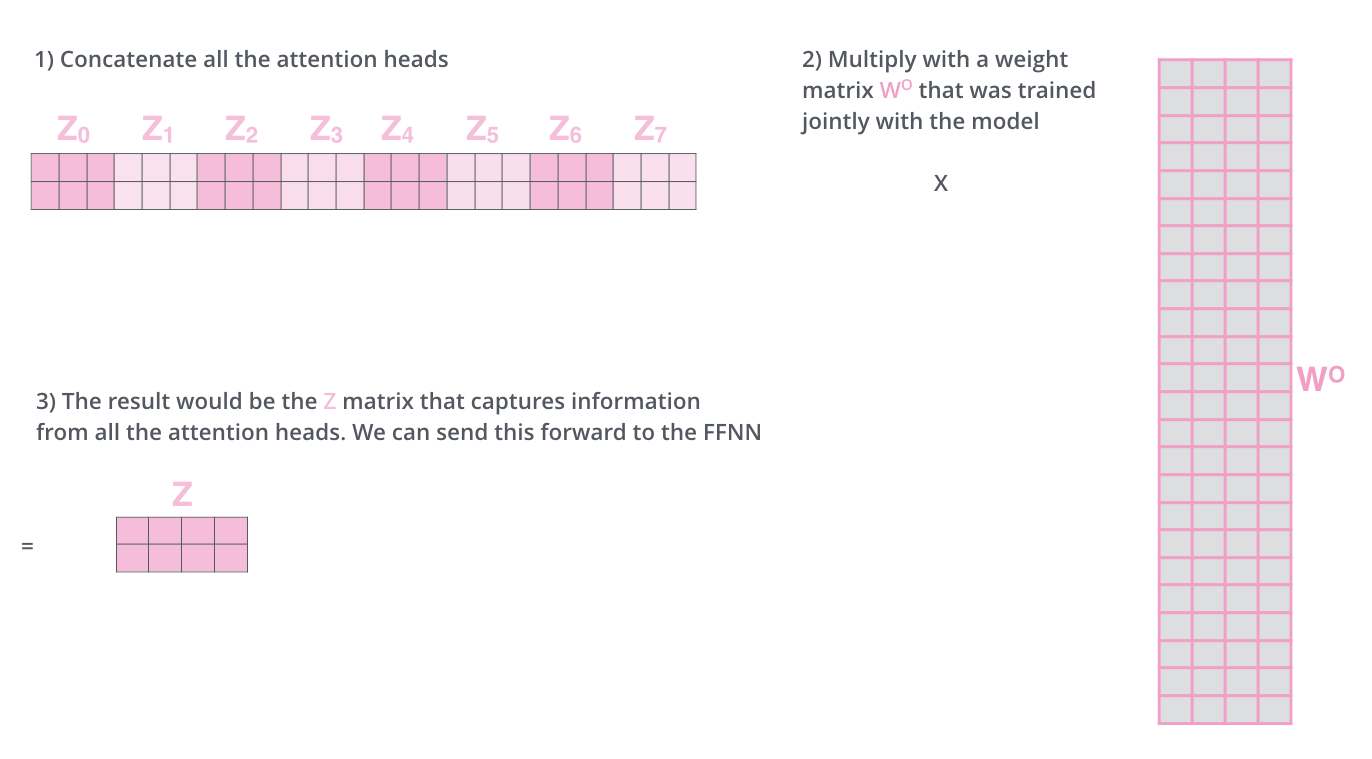
\includegraphics[width=0.85\linewidth]{img/Wo.png}
    \label{fig:placeholder}
\end{figure}

Here is the whole multi-head attention process visually:

\begin{figure}[H]
    \centering
    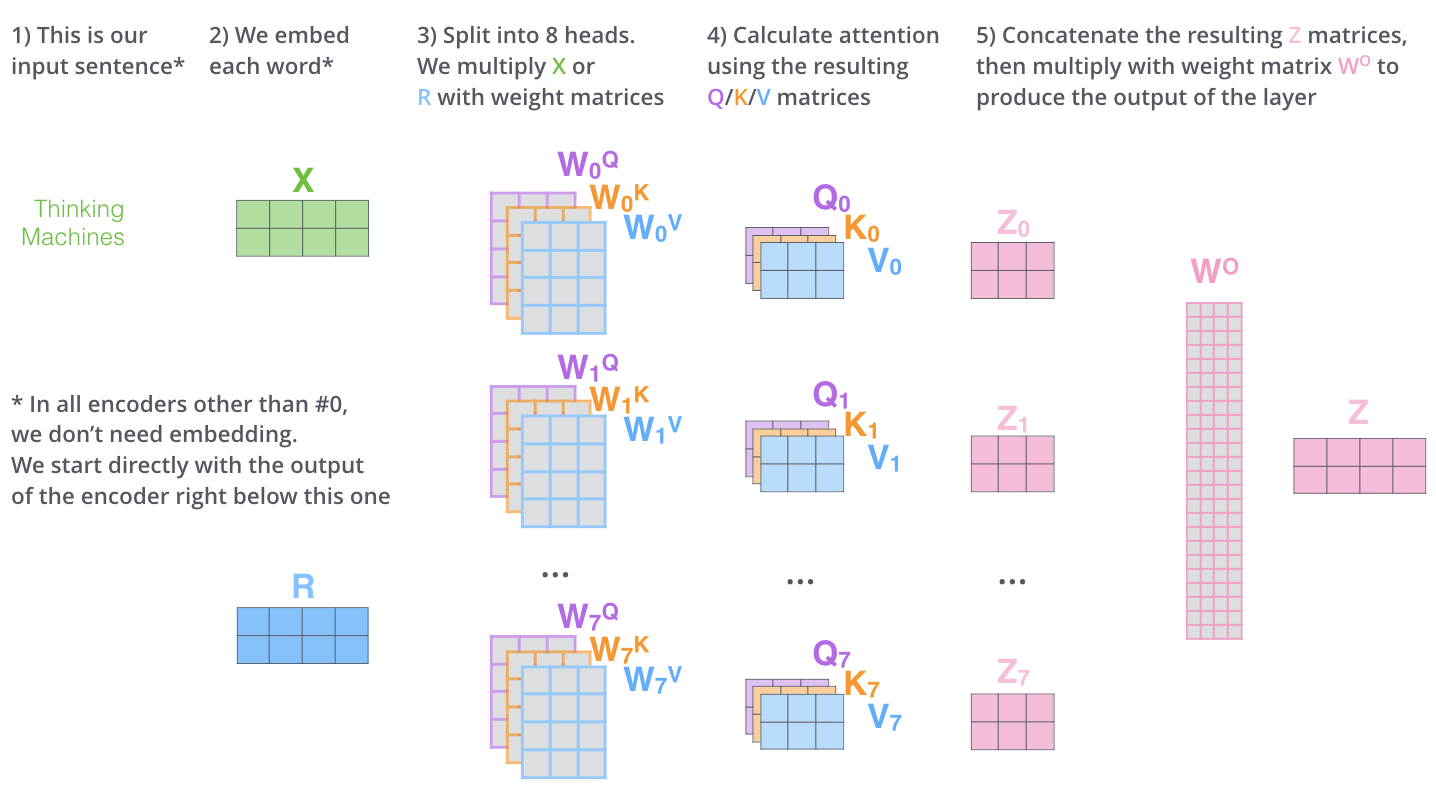
\includegraphics[width=0.85\linewidth]{img/multihead.png}
    \label{fig:placeholder}
\end{figure}

The output is then fed to the FFNN layer, which consists of two linear transformations with a ReLU activation in between. The FFNN is applied to each position separately and identically, meaning that it does not share parameters across different positions in the sequence.

\subsubsection{The Decoder}
The decoder uses the same architecture as the encoder, but with an additional attention layer that attends to the output of the encoder stack, called the "encoder-decoder attention" layer. 

The encoder stack part is responsible for generating a bidirectionally contextualized embedding matrix of the input sequence, the $K$ and $V$ matrices. These are to be used by each decoder in its “encoder-decoder attention” layer which helps the decoder focus on appropriate places in the input sequence.

\begin{figure}[h!]
    \centering
    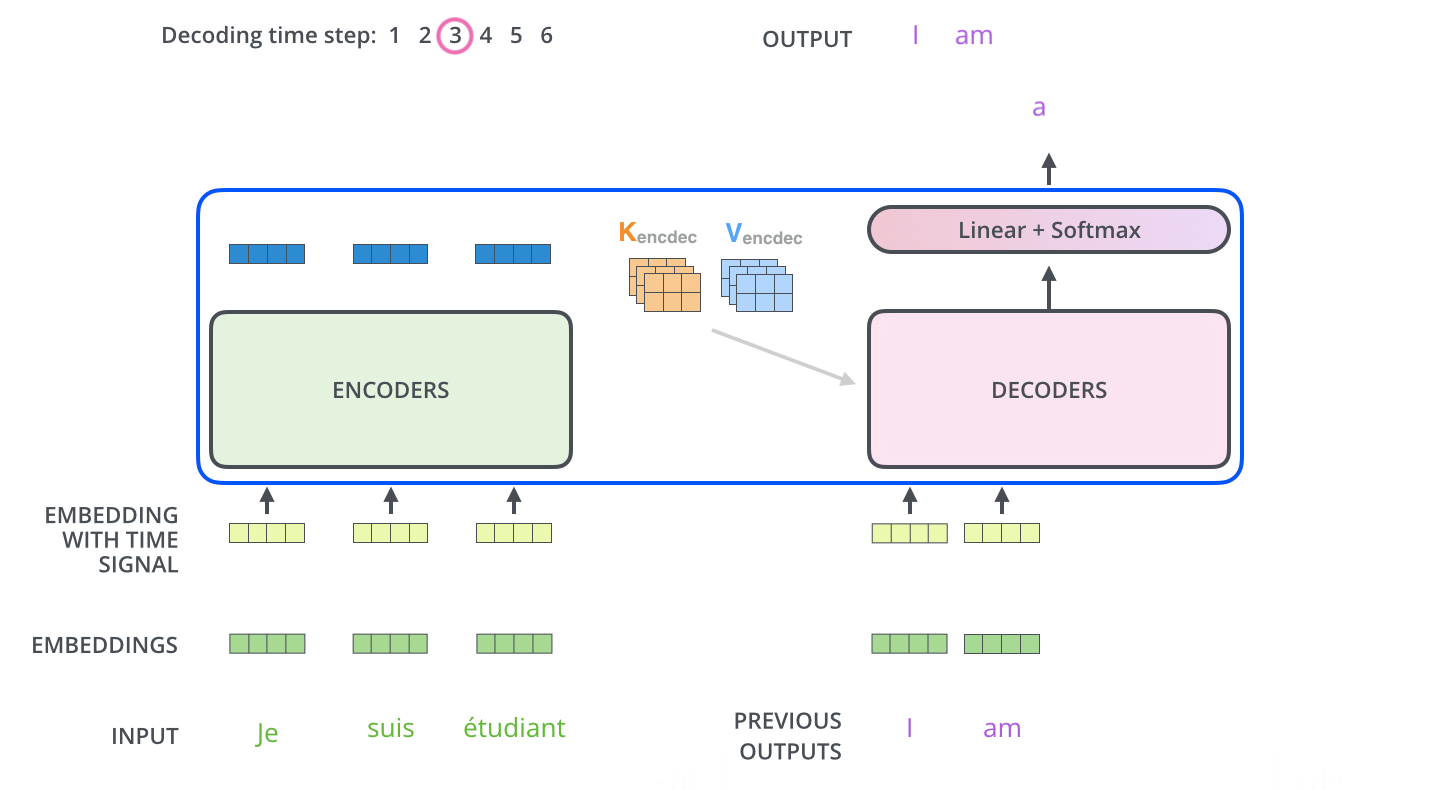
\includegraphics[width=1\linewidth]{img/encdev_attention.png}
    \label{fig:placeholder}
\end{figure}

The following steps repeat the process until a special symbol is reached indicating the transformer decoder has completed its output. The output of each step is fed to the bottom decoder in the next time step, and the decoders bubble up their decoding results just like the encoders did. And just like we did with the encoder inputs, we embed and add positional encoding to those decoder inputs to indicate the position of each word.

In the decoder, the self-attention layer is only allowed to attend to earlier positions in the output sequence. This is done by masking future positions (setting them to -inf) before the softmax step in the self-attention calculation.

The “Encoder-Decoder Attention” layer works just like multiheaded self-attention, except it creates its Queries matrix from the layer below it, and takes the Keys and Values matrix from the output of the encoder stack.

\subsection{The intuition behind Self-Attention}
The self-attention mechanism allows the model to weigh the importance of different tokens in the input sequence when generating a representation for each token. 
When studying the paper, we found the simple use of the $Q$, $K$, and $V$ matrices to be quite elegant at capturing such an simple yet illusive concept. 

As in many DL approaches, the weights of the $W^Q$, $W^K$ and $W^V$ matrices were randomly initialized. During training, the model learns to adjust these weights in such a way that the resulting $Q$, $K$, and $V$ matrices capture the necessary information to compute meaningful attention scores.

\begin{itemize}
    \item [$Q$:] The query vector essentially represents what the current token asks of the rest, in order to narrow down its meaning. For example, the token "bank" can have two representations, one for the financial institution meaning and one for the river bank meaning. The query vector for "bank" would learn to "ask" the rest of the tokens if they have anything to do with a river or money, in an attempt to narrow down its own meaning. If the context is "I went to the bank to withdraw money", the query vector would learn to ask for information related to finance, while if the context is "The river bank was flooded", it would learn to ask for information related to geography. By the end of training the Query vector for "bank" would have learned to ask the right questions to narrow down its meaning in different contexts.
    
    \item[$K$:] The key vector represents a \textit{summary of what each token has to offer}, optimized for being found by the right queries. It does not carry the full meaning of the token, but rather acts as a label for retrieval. In our example, the token "money" would have a key vector that signals financial relevance, making it a strong match for a query like the one "bank" would produce in a financial context.

    \item[$V$:] The value vector represents the \textit{actual content} that each token contributes once the attention scores have been computed. While the key vector determines how much attention a token receives, the value vector determines what that token actually passes forward. The two are kept separate because being findable and being informative are different tasks, the model can learn to make "money" easy to retrieve via its key, while encoding richer semantic content in its value to blend into the output representation.

\end{itemize}

\subsection{Impact of the Transformer Paradigm}
The introduction of the Transformer architecture represented a seismic shift in Natural Language Processing, moving the field from a sequential "memory-based" approach to a parallelized "attention-based" framework. The impact of this transition can be categorized into three primary dimensions:

\begin{itemize}
    \item \textbf{Computational Scalability:} By discarding the linear dependency of $h_{t}$ on $h_{t-1}$ found in RNNs, the Transformer allowed for massive parallelization across GPU hardware. This enabled the scaling of models to billions of parameters, a feat previously impossible due to the sequential bottleneck.
    \item \textbf{Universal Contextualization:} Unlike LSTMs, where semantic signals often diluted over distance, the self-attention mechanism established a direct, constant-time connection between all tokens in a sequence. This resulted in a more robust and stable semantic manifold, where the representation of a word is strictly tied to its global context rather than its local neighbors.
    \item \textbf{The Birth of Transfer Learning:} Perhaps the most significant impact was the decoupling of \textit{pre-training} from \textit{fine-tuning}. The Transformer provided a general-purpose "backbone" that could learn universal linguistic features from unlabelled data, which could then be specialized for diverse downstream tasks like sentiment analysis or question answering.
\end{itemize}

\section{Bidirectional Encoder Representations from Transformers (BERT)}
As the field's understanding grew on how to better conceive representation of words and sentences and their underlying meaning, so did the scientific research around it. Just a year after the release of the paper that proposed the Transformer architecture, \cite{devlin2019bert} published "BERT: Pre-training of Deep Bidirectional Transformers for Language Understanding".

\subsection{Previous Work and Major Concept}
Before we dive deeper in the architecture behind BERT, let's see a number of clever ideas where it got its inspiration from:

\begin{itemize}
    \item \textbf{Transformer}: A rebellious idea in the NLP world, that replaced the heavily-used LSTM architecture. The consistency of its 2 major parts, the Encoder and the Decoder, alongside with the embedded groundbreaking Attention mechanism, resulted in a never-seen before experimental evaluation.
    \item \textbf{ELMo}: ELMo (Embeddings for Language Models) provided a significant step towards pre-training in the context of NLP, as it introduced both the contextualized embedding for each word and the bi-directional 'scanning' for finding context.
    \item \textbf{ULM-FiT}: Transfer learning methods to effectively utilize what the models learned during pre-training, in order to fine-tune language models for various tasks.
    \item \textbf{OpenAI Transformer}: By using only the Decoder of the Transformer architecture and masking future tokens to predict next words, it handles various downstream tasks.
\end{itemize}

BERT uses the best features of the above to create a new architecture. The authors took advantage of the Transformer by 'stealing' its Encoder and by combining it with ELMo's bi-directioniality and OpenAI's masking technique, they proposed a robust framework, whose experimental evaluation broke records amongst other language models, back when it was published.

\subsection{Diving deeper into the BERT Framework and Architecture}
BERT's model architecture consists of  a multi-layer bidirectional Transformer encoder and there are 2 model sizes proposed:

\begin{enumerate}
    \item \textbf{BERT Base}: Comparable in size to the OpenAI Transformer for performance comparison
    \item \textbf{BERT Large}: A quite larger model, developed to achieve state of the art results
\end{enumerate}


Before talking about the main steps, let's analyze the Input and Output Representations. 
For every sentence (token sequence) given as  \textbf{Input}, the first input token is always the special \textbf{[CLS]} token, which helps us with sentence classification tasks. If we want to split our token sequence in 2 distinct sequences, e.g. for Two-Sentence Tasks, we can use the special token \textbf{[SEP]} to seperate them. As an \textbf{Output}, each position outputs a vector. For the sentence classification task we mentioned before, ouputs from the [CLS] token onward are going to be passed through a classification head which would then yield us our results. \\

\begin{figure}[H]
    \centering
    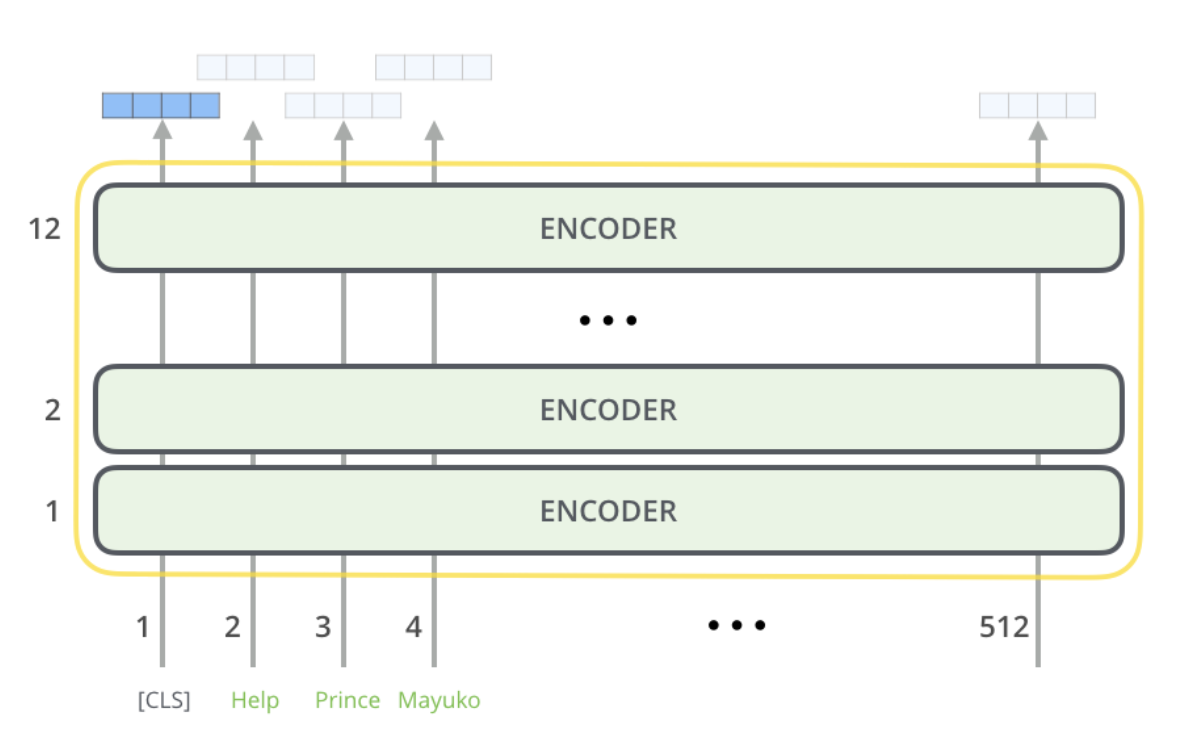
\includegraphics[width=0.85\linewidth]{img/BERT_input_output.png}
    \caption{BERT's Input and Output Representations}
    \label{fig:placeholder}
\end{figure}

Finally, there are 2 steps in BERT's framework, \textbf{Pre-Training} and \textbf{Fine-Tuning}: 

\subsubsection{Pre-Training}
The model is trained on large amounts of unlabeled data, in order to achieve language processing abilities based on the training data set's patterns. Because of the fact that this model is bi-directional, words in a sequence should be treated with extreme caution, as it is possible that each word could see itself and therefore it would trivially predict the next word. The authors deal with this problem with a technique called \textbf{Masked Language Model (MLM)}, where 15\% of tokens are randomly masked for the model to predict. To avoid mismatches between the Pre-Training and Fine-Tuning step, of this 15\%, the 80\% of tokens are replaced with the special \textbf{[MASK]} token, the 10\% with a random token and the rest 10\% remain unchanged.

\begin{figure}[H]
    \centering
    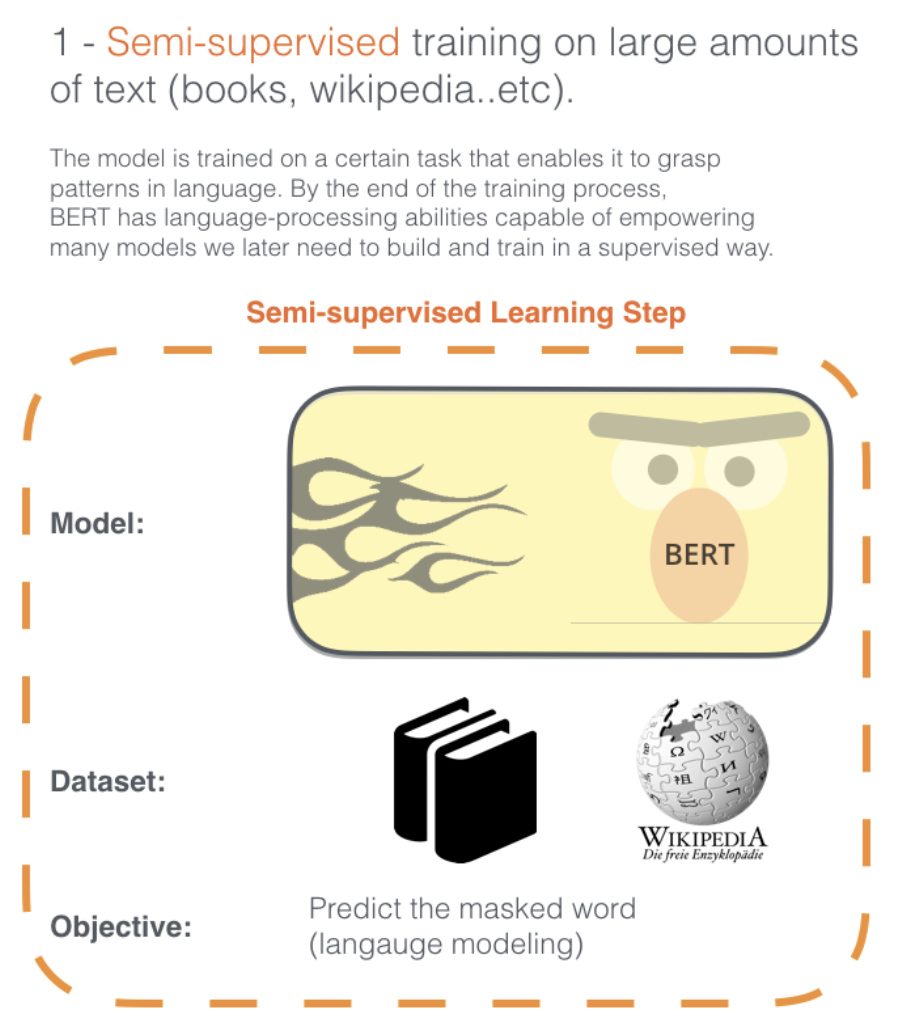
\includegraphics[width=0.85\linewidth]{img/BERT_pre_training.png}
    \caption{BERT'S Pre-Training Phase}
    \label{fig:placeholder}
\end{figure}

\subsubsection{Fine-Tuning}
Since we already have the parameters ready from the Pre-Training Phase, we simply 'plug-in' the task-specific inputs and outputs in our model and let it fine-tune all the parameters. Some of the downstream tasks that our model can fine tune to are: 

\begin{enumerate}
    \item \textbf{Sentence Pair Classification Tasks}
    \item \textbf{Single Sentence Classification Tasks}
    \item \textbf{Question Answering Tasks}
    \item \textbf{Single Sentence Tagging Tasks}
\end{enumerate}

\begin{figure}[H]
    \centering
    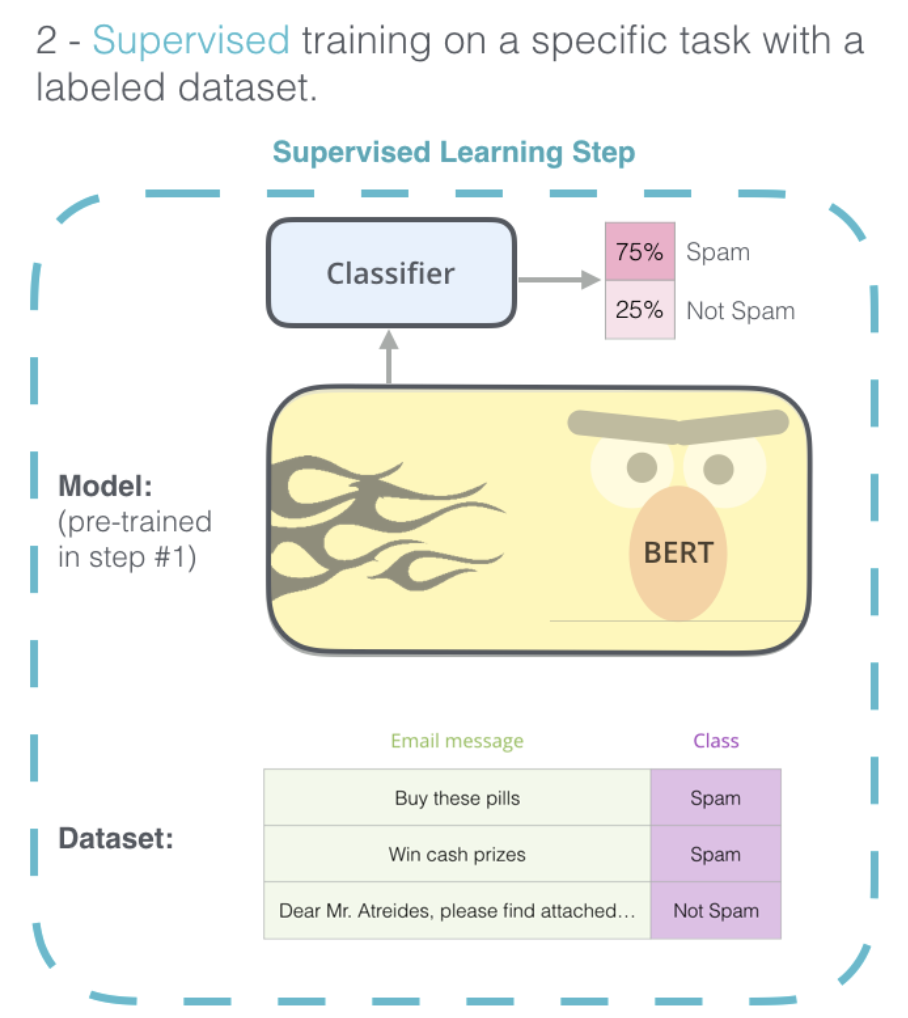
\includegraphics[width=0.85\linewidth]{img/BERT_fine_tuning.png}
    \caption{BERT's Fine-Tuning Phase}
    \label{fig:placeholder}
\end{figure}

\begin{figure}[H]
    \centering
    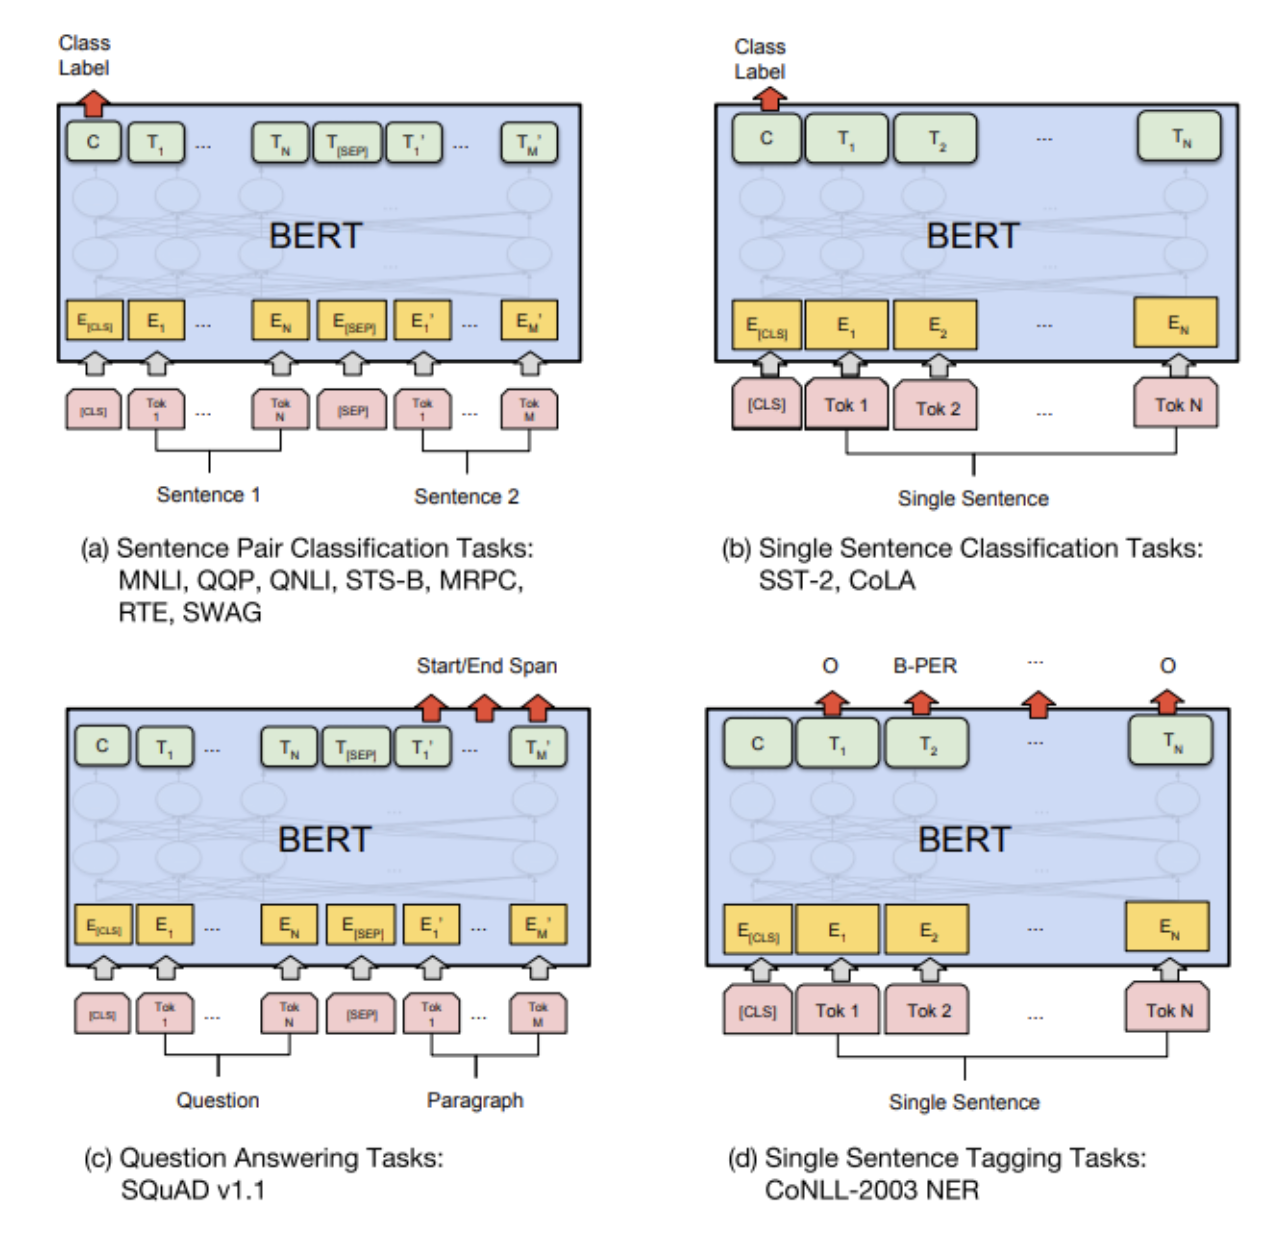
\includegraphics[width=0.85\linewidth]{img/BERT_downstream_tasks.png}
    \caption{Various Downstream Tasks for Fine-Tuning with BERT}
    \label{fig:placeholder}
\end{figure}

\section{TSAPM-BERT: Parametric Refinement for Emotion Prediction}
\label{sec:tsapm}

\subsection{Beyond Sentiment: Mapping the Emotion Manifold}

While traditional sentiment analysis (SA) focuses on the binary or ternary classification of text into positive, negative, or neutral polarities \citep{kayal2026parametrically}, emotion detection seeks a higher level of granularity by identifying specific affective states. The TSAPM-BERT framework operates on an emotion space defined by six distinct classes: \textit{Sadness, Anger, Fear, Joy, Love,} and \textit{Surprise}.

In a standard BERT embedding space, these emotions often overlap because they share similar semantic contexts (e.g., "fear" and "anger" both appearing in negative contexts). Traditional models often flatten this manifold into a simple binary axis, but TSAPM-BERT uses its parametric modifications to warp the semantic space, creating clearer boundaries between these nuanced states.

By mapping these six classes to binary labels, converting Joy, Love, and Surprise to positive (1) and Sadness, Anger, and Fear to negative (0), the researchers demonstrate that a model with high emotional intelligence is inherently better at basic sentiment tasks. The goal of the parametric refinement is to ensure the model captures the "intensity" and "flavor" of the emotion, rather than just its general polarity.

\subsection{Architectural Modification: The $\alpha$ and $\beta$ Parameters}
% This is where we will work on the math of the attention and hidden state.
To enhance the model's focus on emotionally charged vocabulary, the paper proposes a modification of the original BERT's parameters. Specifically, a modification of the attention formula ($A$), as well as the hidden state formula ($H$).

This happens with the help of external sentiment lexicons and polarity score dictionaries from sources like SentiWordNet. 

While the use of such dictionaries isn't novel in and of itself, the injection of them in the parameter level is. Most literature regarding the topic of SA includes these lexicon based approaches on the auxiliary level, thus not providing fine grained emotion understanding capabilities to the model.

\subsubsection{Parametric Attention Modification ($\alpha$)}
Here the authors propose a modification of the original attention formula as follows;

\begin{equation}
    A' = \alpha A_{std} + (1 - \alpha)A_{sent}
\end{equation}

\begin{enumerate}
    \item $A_{std}$ represents the original attention scores obtained from the pre-trained BERT's transformer layers
    \item $A_{sent}$ denotes the sentiment-weighted attention, where sentiment lexicons and polarity scores are used to scale the attention given to sentiment-rich tokens.
    \item $\alpha \in [0, 1]$ is a tunable hyperparameter controlling the balance between the original contextual attention and the sentiment-weighted component.
\end{enumerate}

This sentiment-aware attention $A'$ is designed
to emphasize sentiment-bearing tokens while retaining the contextual dependencies learned by BERT. This approach ensures that tokens with strong emotional or opinionated cues are attended to in a proportionally higher degree than standard tokens, during the encoding process.

By fixing $\alpha$, the researchers ensure that the "emotional signal" is consistently prioritized during the initial phases of the manifold construction, preventing the model from reverting to a generic, non-emotional state.

\subsubsection{Intuition: Lexicon-Guided Latent Representations}
% Explain why injecting Slex vectors "warps" the manifold in a useful way.
Unlike the tunable $\alpha$, the $\beta$ parameter is a \textit{learnable weight} that is optimized during the fine-tuning process. It governs the integration of external sentiment-bearing features from the $S_{lex}$ (Sentiment Lexicon) into BERT's hidden states ($H$). The refined hidden representation $H'$ is calculated as:

\begin{equation}
    H' = H_{std} + \beta \cdot S_{lex}
\end{equation}

$S_{lex}$ is sentiment-bearing vector constructed by mapping the polarity score (positive, negative, neutral) obtained from \textbf{SentiWordNet} for each token, to a fixed-dimensional vector aligned with BERT’s hidden state dimension.

This sentiment-bearing feature vector is injected into the models hidden state before the first Transformer block but after the initial embedding layer. This means that the input of the first Transformer block is essentially the sum of the following:

\begin{itemize}
    \item The initial \textit{token embedding}, obtained likely through an embedding layer such as WordPiece.
    \item The \textit{segment embedding} that distinguishes between various units of text, such as separate sentences or paragraphs, within the input sequence.
    \item The \textit{positional embedding} that captures the sequential order of tokens, allowing the transformer to understand the importance of word order in variable-length sequences.
    \item The $S_{lex}$ vector, derived from external lexicons (SentiWordNet) to provide explicit polarity cues, which is scaled by the learnable weight β and added to the previous three components to form the refined hidden state $H'$.
\end{itemize}

Intuitively, it is as if the researchers give a hint to the model before it begins the self-attention process, about the emotional weight of the word in and of itself, which will then later get refined through by attending to the rest of the tokens in the input sequence.

Through the optimization of $\beta$, the model dynamically adjusts the "injection strength" of emotional metadata. This allows for a more fluid and adaptive refinement of the latent representations, where the model learns the optimal "mixture" of textual context and external emotional knowledge.

\subsection{Training Protocol and Hyperparameter Configuration}

The fine-tuning of the TSAPM-BERT model was conducted using a selective optimization strategy rather than a uniform update of all weights. By targeting specific layers, namely the attention, feed-forward, and embedding layers selectively rather than uniformly, the researchers aimed to balance the preservation of BERT's pre-trained linguistic knowledge with the injection of task-specific emotional metadata.

The above approach was crucial. As the subsequent ablation studies demonstrate, the ability to freeze specific layers while selectively updating others, allowed for more fine grained optimization. This prevented the model from losing its pre-trained semantic foundations, a common failure point in the more coarse-grained, uniform fine-tuning methods typically employed in prior literature

To ensure stable convergence and prevent the model from forgetting general semantic context, the following configurations were implemented:

\begin{itemize}
    \item \textbf{Optimizer:} The \textit{AdamW} optimizer was utilized with a weight decay of 0.01. This variant of the Adam optimizer is specifically chosen for Transformer models to provide better regularization by decoupling weight decay from the gradient update.
    \item \textbf{Learning Rate Management:} A conservative learning rate of $2 \times 10^{-5}$ was paired with 500 warmup steps to facilitate gradual convergence in the early stages of training
    \item \textbf{Regularization:} A dropout rate of 0.3 was applied across the modified layers to mitigate the risk of overfitting.
    \item \textbf{Batch and Epochs:} The model was trained for 5 epochs with a batch size of 32, allowing for a thorough refinement of the $\beta$ parameter without over-exposure to the training set.
\end{itemize}

The specific hyperparameter values are summarized in Table \ref{tab:hyperparameters}.

\begin{table}[H]
\centering
\caption{TSAPM-BERT Hyperparameter Settings}
\label{tab:hyperparameters}
\begin{tabular}{|l|l|}
\hline
\textbf{Hyperparameter} & \textbf{Value} \\ \hline
Learning Rate           & $2 \times 10^{-5}$ \\ \hline
Dropout Rate            & 0.3 \\ \hline
Batch Size              & 32 \\ \hline
Number of Epochs        & 5 \\ \hline
Optimizer               & AdamW  \\ \hline
Max Sequence Length     & 128 tokens  \\ \hline
Warmup Steps            & 500  \\ \hline
Weight Decay            & 0.01  \\ \hline
\end{tabular}
\end{table}

This targeted fine-tuning approach successfully minimized the overfitting gap to approximately 0.85\%, as evidenced by the convergence of the training (99.37\%) and testing (98.52\%) accuracies.

\subsection{Performance Evaluation and Ablation Analysis}

\subsubsection{The Fine-Tuning Dataset}
The model was trained and tested on an emotion dataset containing 18,000 rows, 9,725 unique tokens and six total emotion classes. Namely: Sadness, Anger, Fear, Joy, Love and Surprise. 

A Training/Validation/Test split of 70/10/20 was used, along with a 5-fold cross-validation strategy to ensure unbiased and robust performance estimation.

Performance was measured through a comprehensive suite of metrics, including Accuracy, Precision, Recall, F1-score, Sensitivity, and Specificity. Statistical significance was further validated through pairwise t-tests, confirming that the improvements offered by TSAPM-BERT were not the result of random chance.

\subsubsection{Comparative Results}
TSAPM-BERT achieved state-of-the-art results, significantly outperforming traditional machine learning, ensemble, and deep learning baselines, as well as other SOTA BERT models fine-tuned for the same task.

\begin{itemize}
    \item {\textbf{Accuracy: }}The model achieved a $99.37\%$  training accuracy and a $98.52\%$ testing accuracy.
    \item {\textbf{Generalization: }}While baseline models like Naive Bayes achieved near-zero overfitting gaps, they did so at the cost of lower overall accuracy. TSAPM-BERT achieved a superior testing accuracy of $98.52\%$ while maintaining a minimal overfitting gap of $0.85\%$, indicating that the parametric modifications successfully regularized the high-capacity Transformer architecture
\end{itemize}

\begin{figure}[h!]
    \centering
    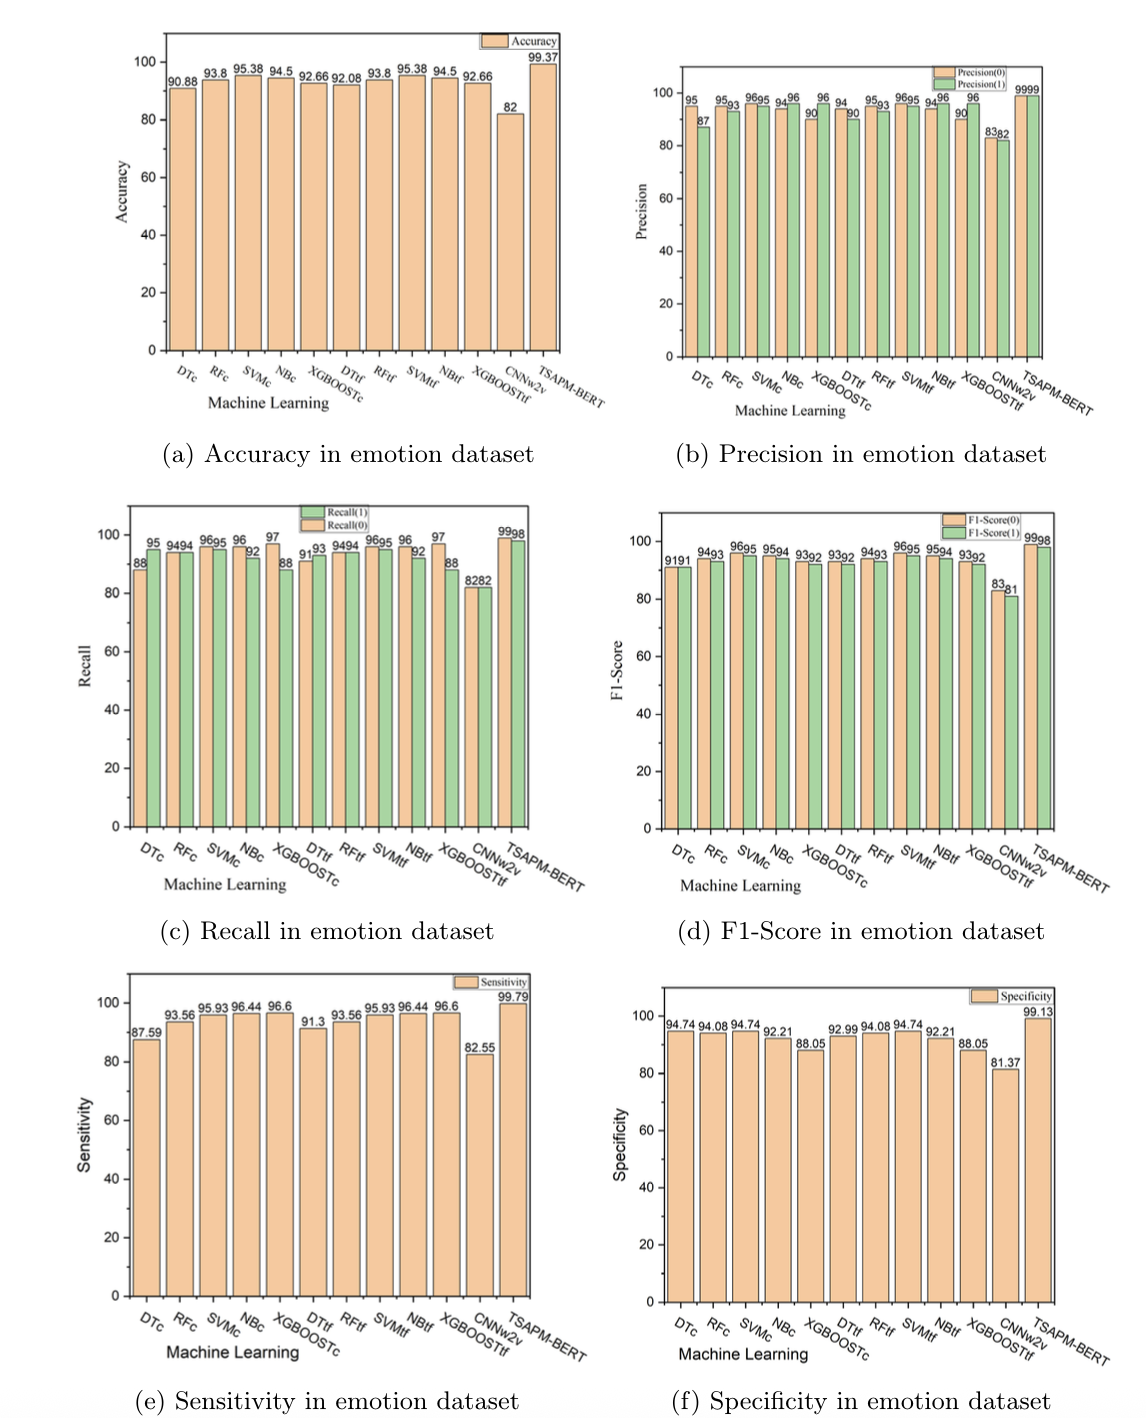
\includegraphics[width=1\linewidth]{img/acc.png}
    \caption{Performance metrics}
\end{figure}

Results on the CARER dataset when pitted against the other SOTA BERT models also showed superior results, demonstrating the effectiveness of the authors' proposed hybrid architecture and its strong generalization ability over existing sentiment and emotion classification methods. ***


\subsection{Ablation Analysis: Quantifying Parametric Impact}

To validate the structural necessity of the TSAPM-BERT modifications, the researchers conducted a series of ablation studies. These experiments systematically removed specific components to observe the resulting degradation in predictive performance.

\subsubsection{Impact of Sentiment Lexicon ($S_{lex}$)}
The first setting involved removing the sentiment-aware vector $S_{lex}$ ($\beta = 0$), forcing the model to rely solely on the contextual embeddings generated by standard BERT.

\begin{itemize}
    \item \textbf{Result:} A noticeable drop in accuracy, precision, recall, and F1-score across all classes
    \item \textbf{Intuition:} This degradation indicates that while standard BERT is highly effective at capturing general semantic context, it lacks explicit sensitivity to emotional polarity. The absence of $S_{lex}$ particularly hindered the model's ability to distinguish subtle affective expressions in short or ambiguous texts.
\end{itemize}


\subsubsection{Effect of Weighted Attention Refinement ($\alpha$)}
In this setting, the weighted attention mechanism was disabled by setting $\alpha = 1$, reverting the model to standard self-attention without sentiment-guided emphasis.

\begin{itemize}
    \item \textbf{Result:} A consistent reduction in Recall and F1-score, with the most significant impact observed in \textit{minority emotion classes} (e.g., Fear or Surprise)
    \item \textbf{Intuition:} Without the weighted refinement, the model tends to distribute attention focus too uniformly across tokens, effectively diluting the influence of emotionally salient words. This confirms that $\alpha$ successfully guides the model to prioritize "emotionally informative" regions of the text.
\end{itemize}

\subsubsection{Parametric vs. Uniform Fine-Tuning}
Finally, the researchers replaced TSAPM-BERT with a standard fine-tuned BERT model, removing the parameters $\alpha$ and $\beta$ entirely and applying uniform fine-tuning.

\begin{itemize}
    \item \textbf{Result:} This configuration resulted in the \textbf{largest performance decline} of all ablation settings.
    \item \textbf{Overfitting Analysis:} Crucially, this version showed a significantly increased overfitting gap. This proves that parametric control ($\alpha, \beta$) allows for a more stable learning process by balancing general pre-trained knowledge with task-specific emotional signals.
\end{itemize}

\begin{table}[h]
\centering
\caption{Summary of Ablation Study Impacts}
\label{tab:ablation}
\begin{tabular}{|l|l|}
\hline
\textbf{Setting Removed} & \textbf{Primary Consequence} \\ \hline
Sentiment Lexicon ($S_{lex}$) & Loss of sensitivity to emotional polarity  \\ \hline
Weighted Attention ($\alpha$) & Focus dilution; drop in minority class F1-scores \\ \hline
Parametric Control ($\alpha, \beta$) & Largest accuracy drop; increased overfitting gap \\ \hline
\end{tabular}
\end{table}

\subsection{Summary of Contributions}

The primary contribution of the TSAPM-BERT framework is the demonstration that BERT's general-purpose architecture can be surgically modified to excel in niche, high-granularity tasks like emotion prediction. By moving away from uniform fine-tuning and instead utilizing the hyperparameter $\alpha$ and learnable $\beta$ parameters to integrate external sentiment lexicons, the model achieved a state-of-the-art testing accuracy of 98.52\%. 

The success of this approach lies in its "emotionally informed" representations, which provide a robust solution for interpreting the ambiguous and often sarcastic nature of social media data. For the purposes of this report, TSAPM-BERT serves as a benchmark for how external domain knowledge can be fused with pre-trained transformer architectures to push the boundaries of Natural Language Understanding.

\subsection{Critical Analysis: Benchmarking and Domain Constraints}

While the TSAPM-BERT model demonstrates a numerically superior accuracy of 98.52\%, a critical review of the comparative analysis in Table 7 of the paper reveals a significant methodological limitation. The authors primarily compare their results against other models evaluated on the CARER dataset; however, the most recent direct comparison provided for this specific dataset dates back to 2018 \citep{saravia2018carer}. 

Furthermore, while the paper cites state-of-the-art (SOTA) models from 2024 and 2025, these were evaluated on disparate datasets such as the "Restaurant" domain \citep{zhao2025aspect}. Because emotional and linguistic manifolds vary drastically across different domains, this cross-dataset comparison lacks the "apples-to-apples" rigor required for a definitive claim of global superiority. Additionally, although the authors advocate for the model's adaptability, the current study lacks the cross-domain or multilingual validation they suggest for future research. This indicates that while the parametric modifications are highly effective for the CARER vector space, their universal applicability remains to be empirically proven.


\clearpage
\section{RexBERT: Domain Specialization through Data Curation}
\label{sec:rexbert}

\subsection{Motivation: The E-commerce Domain Gap}
While general-purpose encoders like BERT and ModernBERT \citep{warner2025smarter} provide robust linguistic foundations, they often struggle with the unique structural and semantic properties of the e-commerce domain. Retail language is characterized by high entity density, semi-structured attribute-value pairs (e.g., "Screen Size: 6.5 inches"), and complex polysemy where product substitutes and complements must be mathematically distinguished. RexBERT was developed to bridge this gap by prioritizing high-quality in-domain data and a principled training curriculum over indiscriminate parameter scaling.

\subsection{The Ecom-niverse Corpus: Distillation at Scale}
The primary asset enabling RexBERT's specialization is \textit{Ecom-niverse}, a curated 350-billion-token corpus derived from the 4.4-trillion-token FineFineWeb collection. To isolate commerce-relevant text from general web noise, the authors employed a modular curation pipeline:

The FineFineWeb collection contains entries of text and their respective domain labels. Because of the small number of possible labels, the authors manually split the categories that exhibit relevance to the e-commerce domain, into two categories. The "Directly Selected" ones, and the "Filter required" ones. The "Directly Selected" category involved categories with near-complete overlap with e-commerce, such as Fashion/Beauty (15.3\%). The ones requiring filtering presented less of overlap, such as "News" (11.7\%) and "Health" (8.4\%),

Their proposed data curation pipeline is described as follows:
\begin{itemize}
    \item \textbf{Sampling:} A sampling strategy was used to select a smaller yet representative subset of items from each relevant domain category, ensuring a manageable volume for manual annotation while preserving the diversity of the original corpus.
    \item \textbf{Instruction-Tuning:} A smaller, instruction-tuned model (Phi-4) was used to assign binary "Relevant/Not Relevant" labels to sampled items, while a stronger model (Llama3-70B) audited these labels for consistency.
    \item \textbf{FastText Distillation:} These high-quality labels were distilled into scalable fastText classifiers. This process distills the essential classification logic of the much heavier LLMs into a much smaller and more efficient fastText classifier, enabling the high-throughput scoring and thresholded filtering of the entire corpus of each of the selected relevant domains.
    \item \textbf{Classifier Validation:} Each classifier is validated with held-out evaluation and/or cross-validation to assess generalization within its domain and to calibrate score distributions.
    \item \textbf{Corpus Assembly:} Finally, the validated fastText models are applied at scale to their corresponding FineFineWeb domain partitions, producing relevance scores for all items; a domain-wise threshold on these scores yields the retained subset, resulting in a validated, e-commerce focused corpus for pre-training.
    
\end{itemize}

\begin{figure}[h!]
    \centering
    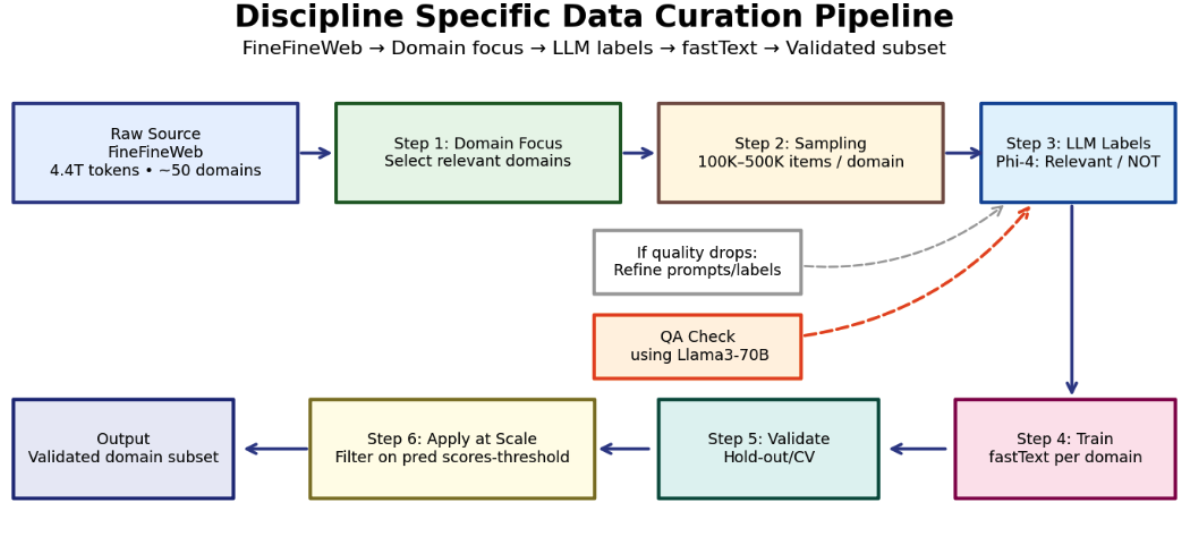
\includegraphics[width=0.75\linewidth]{img/rex_cleaning_pipeline.png}
    \caption{Ecom-niverse curation pipeline}
    \label{fig:placeholder}
\end{figure}

While RexBERT categorizes its target domains into 'Directly Selected' and 'Filter Required,' the subsequent pipeline treats these groups with identical algorithmic rigor. This categorization appears to be a descriptive framework for characterizing source purity and justifying the need for domain-conditioned filters, rather than an operational branching in the curation logic

\subsection{Architectural Foundation: ModernBERT Integration}
RexBERT utilizes a BERT-style encoder that incorporates several transformative enhancements from the ModernBERT architecture \citep{warner2025smarter}. These modifications are designed to optimize the semantic manifold's efficiency, stability, and context-handling capabilities:

\begin{itemize}
    \item \textbf{Biasless Layers and Pre-normalization:} The authors removed the bias terms from the linear layers. In addition, while the original BERT architecture utilized Post-Layer Normalization, effectively normalizing the residual sum at the exit of each sublayer, RexBERT adopts a Pre-Norm configuration. This ensures that the primary residual branch remains un-normalized, providing a more stable 'gradient highway' that facilitates the training of deeper architectures like RexBERT-Large. These changes follow ModernBert's initiative to use the saved compute towards another purpose such as deeper architectures and longer training for the same budget, and maintaining training stability in deep architectures by preventing gradient instability.
    \item \textbf{Rotary Positional Embeddings (RoPE):} Moving beyond the absolute positional embeddings of the original BERT, RexBERT adopts RoPE. RoPE lets transformers understand relative positions naturally and generalize to longer sequences without retraining or extra parameters.
    \item \textbf{GeGLU Activations:} The model replaces standard GELU activations with Gated Linear Units (GeGLU), which provide superior optimization performance and a more expressive latent space.
    \item \textbf{Alternating Global and Local Attention:} Standard attention has a quadratic $O(N^2)$ complexity, making it too slow for RexBERT's 8,192 token sequences. To solve this, the model alternates between local sliding windows, which only process nearby tokens to save compute, and full global layers that maintain the big picture context. This hybrid design allows the model to process long product descriptions efficiently without losing the ability to connect distant pieces of information.
    \item \textbf{Unpadding and Flash Attention:} Standard BERT models waste significant computation by processing the so called padding tokens in sequences shorter than the maximum length. RexBERT adopts unpadding to strip away these filler tokens, ensuring the GPU only processes actual data. Combined with Flash Attention, which is a hardware-aware implementation that accelerates the attention calculation, the model achieves a much higher throughput than the original architecture.
    \item \textbf{Hardware-Aware Depth:} The Micro, Mini, Base and Large variants follow a deep-and-narrow design to maximize GPU utilization within parameter budgets
\end{itemize}

\subsection{The Three-Phase Pre-training Recipe}
RexBERT avoids the pitfalls of "from-scratch" domain training by utilizing a three-phase curriculum designed to build a stable semantic vector space before introducing specialized retail complexity. This curriculum functions as a staged progression that prevents catastrophic forgetting while expanding the model's contextual horizon.

\begin{itemize}
    \item \textbf{Phase 1: General Foundation (1.7T Tokens):} The model begins with a broad "diet" of 1.7 trillion tokens encompassing web text, code, and multilingual technical papers. This phase uses a shorter sequence length of 512 tokens to maximize computational efficiency and establish robust initial token representations.
    \item \textbf{Phase 2: Context Extension (250B Tokens):} Following the general pre-training, the checkpoint is trained for an additional 250 billion tokens to expand the context window to 8,192 tokens.\footnote{The authors acknowledge that Phases 1 and 2 mirror the Ettin methodology \citep{weller2025seq}, and that Ettin's 8,192-token checkpoint was used as the starting point for Phase 3.} This phase allows the model to generalize to longer sequence scenarios, such as complex product tables and concatenated attribute blocks, which are critical for e-commerce semantics. The authors note that Phases 1 and 2 mirror Ettin's methodology, and they use Ettin's 8,192-token checkpoint as the starting point for Phase 3.
    \item \textbf{Phase 3: Annealed Specialization (350B Tokens):} In the final phase, the model is "annealed" onto the 350-billion-token Ecom-niverse corpus. The sampling distribution is gradually shifted toward retail-specific data, allowing the model to specialize its latent representations for the commerce domain without losing its general linguistic capabilities.
\end{itemize}

\subsection{Guided MLM: Strategic Latent Refinement}
To further refine the latent semantic space during the annealing phase, RexBERT introduces \textit{Guided MLM}, a targeted masking strategy that acts as a domain signal amplifier. While standard BERT architectures mask tokens at random, Guided MLM prioritizes "high-value" spans that carry the most significant structural weight in a retail context

\begin{itemize}
    \item \textbf{Entity and Attribute Targeting:} The pipeline pre-identifies domain-relevant spans, such as brand names, technical specifications, and product attributes, and preferentially masks these elements. This forces the model to learn the compositional logic required to reconstruct complex product descriptors from sparse context.
    \item \textbf{The 5\% Mixture Strategy:} To maintain broad NLU performance, Guided MLM sequences only account for approximately 5\% of each training batch. The remaining 95\% of the batch follows a standard random span-masking scheme, ensuring the model's "generalist" knowledge is preserved while it gains "specialist" expertise.
    \item \textbf{Outcome on Latent Space:} This strategic refinement results in improved ordering of graded relevance in the embedding space, allowing the model to more accurately distinguish between subtle product relationships, such as substitutes versus complements.
\end{itemize}

\subsection{Evaluation: Benchmarks and Pareto Efficiency}
The performance of RexBERT was validated across both general linguistic tasks and domain-specific e-commerce benchmarks. The results demonstrate that a refined training curriculum on high-quality data can supersede raw parameter scaling, moving the model toward the \textit{Pareto frontier} of efficiency.

\begin{table}[h]
\centering
\caption{Comparative performance on e-commerce and general benchmarks.}
\label{tab:rexbert_results}
\begin{tabular}{lccc}
\hline
\textbf{Model} & \textbf{Params} & \textbf{ESCI-token (Avg k=1,3,5)} & \textbf{GLUE (Avg)} \\ \hline
RexBERT-Mini & \textbf{68M} & \textbf{77.52}       & 89.31       \\

ModernBERT-Base & 149M           & 75.13               & 89.90                \\
\textbf{RexBERT-Base} & \textbf{150M} & \textbf{81.22}       & \textbf{90.62}       \\

ModernBERT-Large & 395M           & 78.91               & 92.54               \\
\textbf{RexBERT-Large} & \textbf{400M} & \textbf{83.67}      & \textbf{92.69}       \\ \hline
\end{tabular}
\end{table}

\begin{itemize}
    \item \textbf{E-commerce Specialization (ESCI):} On the Amazon ESCI benchmark, RexBERT-Mini (68M parameters) outperformed models roughly twice its size. This confirms that the training regime of a much smaller model on a high-quality, domain specific dataset, can outweigh the more broadly trained, albeit much bigger, generalist model such as ModernBERT-Base.
    \item \textbf{Generalization (GLUE):} Despite its specialization, RexBERT maintains competitive performance on the GLUE benchmark. This stability is attributed to the 5\% Guided MLM mixture and the phased training approach, which prevents the "forgetting" of general linguistic structures during domain adaptation.s
\end{itemize}

\subsection{Summary of Contributions}
The presented paper contributes the following:

\begin{enumerate}
    \item \textbf{Ecom-niverse:} A curated, high-quality 350B token collection of retail-relevant text. This corpus was distilled from the 4.4T FineFineWeb collection using a domain-conditioned LLM-based curation pipeline, providing a high-quality foundation for e-commerce specialization.
    \item \textbf{A Three-step training regime} based on a modernised encoder architecture. In includes (1) pre-training on a diverse mixture of multiple-domain text (2) context extension to support longer sequences (8,192 tokens), and (3) annealing, which gradually shifts the sampling distribution toward Ecom-niverse and incorporates a Guided MLM masking strategy.
    \item \textbf{Efficiency and Pareto Optimization:} A demonstration that 2--3$\times$ smaller models can outperform significantly larger generalist models on domain-specific benchmarks. Specifically, RexBERT-Mini (68M) achieves higher ESCI accuracy than ModernBERT-Base (149M) while maintaining, and in the case of the Base and Large variants, even surpassing competitive performance on general linguistic tasks (GLUE).
\end{enumerate}

\subsection{Critical Analysis: The Guided MLM Ablation Gap}

While the paper presents Guided MLM as a key innovation for
domain specialization, the authors explicitly acknowledge
that no controlled ablation study was conducted to isolate
its contribution. The observed improvements are described
as ``consistent with the mechanism it targets,'' but the
paper cannot disentangle the marginal effect of Guided MLM
from the concurrent effects of corpus composition and the
annealing schedule. In other words, it remains unclear how
much of RexBERT's domain performance gain stems from
\textit{what} it was trained on (Ecom-niverse) versus
\textit{how} certain tokens were masked during training
(Guided MLM). A straightforward ablation, training an
identical model with standard random masking on the same
corpus and schedule, would be necessary to quantify this.
Until such an experiment is conducted, Guided MLM's
contribution remains a plausible but unverified hypothesis.

\clearpage
\section{Multitask Learning and BERT Embedding for Subjectivity Detection and
Aspect-Based Sentiment Analysis}

\subsection{Review Analysis in the E-Commerce Era}
The majority of communication between merchants and clients online happens through reviews and product feedbacks. For the merchant, it is completely and utterly important to carefully read and analyze the response to what he has been producing. However, the huge amounts of reviews on the internet turn this procedure on something that takes huge amounts of time, so we turn on the need for something automized. Even though sentence-level sentiment analysis 
might seem to be a good fit, it oversees how the real client reacts to a product and that is by focusing on its aspects (e.g. color,price,etc.). That is why researches approached the problem with \textbf{Aspect-Based Sentiment Analysis (ABSA)}, a more aspect-focused approach on classifying a text's sentiment by giving more weight to the 'protagonistic' entities. Alongside this, researches also turn their focus on \textbf{Subjectivity Detection (SD)}. 
We care more for subjective than objective opinions, as by filtering out the objective ones, which by the way can be classified of 'Neural' sentiment, the model assigns fine-grained sentiments only on subjective aspects, thus avoiding its 'confusion' and reducing false positives in sentiment classification. By exploiting multitask learning, this approach tends to prove the generalization achieved by the combination of the 2 tasks and the remarkable 
state-of-the-art results they achieve. The key contributions, as mentioned on the paper, are:

\begin{enumerate}
    \item {Developing a multitask learning model that jointly optimizes subjectivity detection and aspect-level sentiment classification tasks}
    \item {Incorporating subjectivity knowledge through the contextual information and semantic knowledge encoded in BERT embeddings to further boost the performance of the multitask learning model}
    \item {Addressing class imbalance issues by demonstrating that the proposed framework effectively addresses precision-recall imbalance problems}
\end{enumerate}

\subsection{Key Components}
Before we dive deeper into the framework's architecture, we are going to analyze it's key components, both conceptually and technically.
\subsubsection{Aspect-Based Sentiment Analysis (ABSA)}
When we talk about Aspect-Based Sentiment Analysis (ABSA), we want to understand what are the emotions linked to product features or attributes in a document (text,review,etc.). Moreover, we want to realise the impact that these emotions have in the entire document's polarity, which can be positive, neutral or negative. Even though it sounds simple, the challenge to the sentiment classification task arrives when we want to realise how the semantic associations 
develop between the main aspect feature of the sentence and its surrounding contextual elements. Previous papers have defined the key elements for conducting an ABSA research. These are \textbf{Aspect term a}, which is the target of opinion, \textbf{Aspect opinion o}, which is the classification of target, \textbf{Opinion term o}, the sentiment conveying to the opinion about the target and \textbf{Sentiment Polarity p}, the emotional attitude linked to an aspect term.They also define a series 'textbook' ABSA tasks, which we call single ABSA tasks, and their combinations, the compound ABSA tasks. These are:

\begin{enumerate}
    \item \textbf{Aspect Term Extraction (ATE)}
    \item \textbf{Aspect Category Detection (ACD)}
    \item \textbf{Opinion Term Extraction (OTE)}
    \item \textbf{Aspect Sentiment Classification (ASC)}
\end{enumerate}

\begin{figure}[h!]
    \centering
    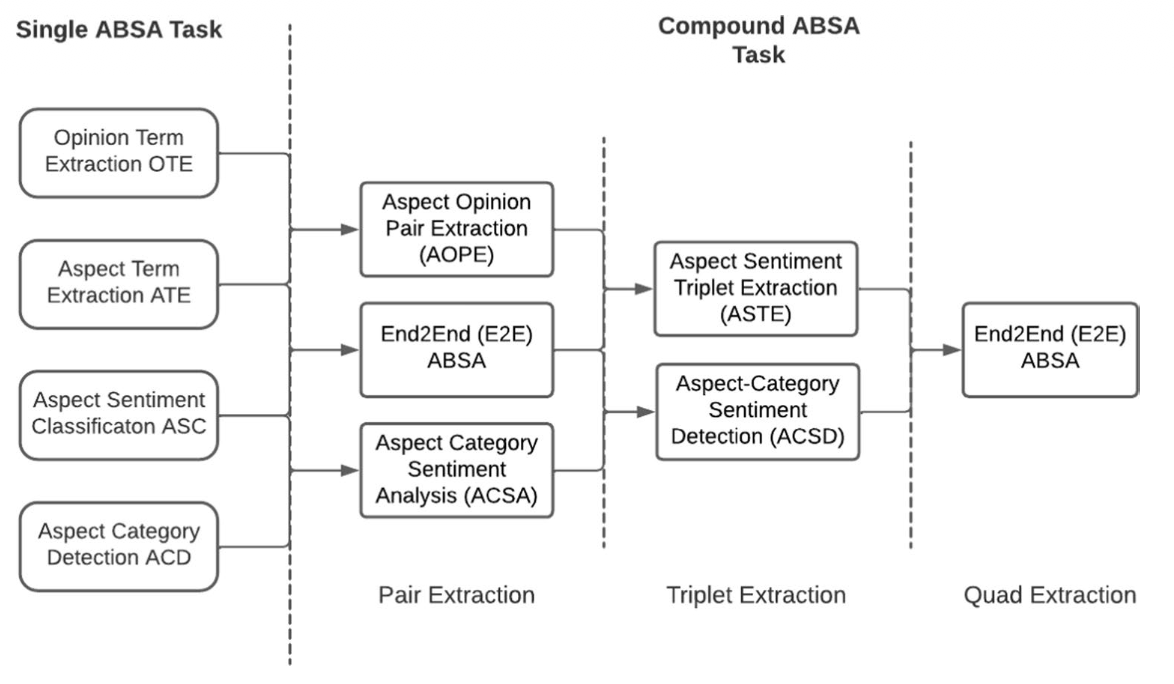
\includegraphics[width=1\linewidth]{img/ABSA_tasks.png}
    \caption{Single and Compound ABSA Tasks}
\end{figure}

The compound ABSA tasks formed by the single ones can be seen on the corresponding image. 

\subsubsection{Subjectivity Detection (SD)}
The objective of Subjectivity Detection (SD) is to distinguish subjective content, which includes personal opinions and emotions of clients about products, from objective content. For example, let's say we have the following online review about a phone : "Its huge 7.9 inch screen cannot fit into my pocket, but I love its bright green color.". Obviously, the screen size is a standard feature that cannot change from phone to phone, thus being characterized as large is objective. On the other hand, the color constant, not only on phones but on any products, is completely subjective, as other clients may find green 
as a repulsive choice for a phone color. Why would the authors want to classify subjectivity alongside ABSA in a single model? The answer is that their intuition drove them to test SD as an auxiliary subtask besides ABSA, with the hope that it will potentially enhance the entire pipeline's performance, by extracting meaningful insights from the document.

\subsubsection{Multitask Learning}
Even though past publications opted for training ABSA subtasks independently from each other, the authors on this paper choose to embrace a Multitask Learning Framework for their research. The reason is that with such framework, the model can learn a shared information representation between tasks, that will potentially enhance the overall performance, especially boosting single tasks more than by training them one at a time. The authors state the 3 reasons written below to justify their choice:

\begin{enumerate}
    \item The shared representations acquired across multiple tasks can facilitate improved generalization.
    \item The mutually beneficial relationships between tasks can enhance the performance of individual tasks during the multitask training process.
    \item A single model capable of handling multiple tasks simultaneously can lead to reduced system complexity.
\end{enumerate}

\subsubsection{BERT Embeddings}
Last but not least, the choice of pre-trained transformer based language models is obvious for various NLP tasks and ABSA is no exclusion. For this experiment, \textbf{Bidirectional Encoder Representation Transformer (BERT)} was chosen, due to its great state-of-the-art results. Its bidirectional Transformer network, which allows for it to look both right and left of the target word to better understand the surrounding context, along with its 2-phase deployment phase (Pre-Training and Fine-Tuning), 
allow it to better capture semantic and syntactic information from the text it is parsing, which are both really important for our ABSA framework as we mentioned before. This is also backed up by previous studies which used transformer-based language models to tackle the ABSA problem and they outperformed the previously used neural architectures.

\subsection{SMABSA Framework}
\subsubsection{Definitions and Notations}
Before we analyze the architecture of \textbf{Subjectivity Multitask Aspect-based Sentiment Analysis (SMABSA)}, let's first see the notations we are going to use. From the previously mentioned single ABSA tasks, the main task that this research studie is \textbf{Aspect Sentiment Classification (ASC)}. The input is a sentence ($S={w_1,w_2,...,w_n}$) and an aspect term withing that sentence ($a={w_i,...,w_j}$) and the output y will be the sentiment polarity of a in S ($y \in \{positive,neutral,negative\}$). The auxiliary task of Subjectivity Detection aims to mark the same aspect term a with a binary label z (0 for objectivity, 1 for subjectivity). These 2 tasks are jointly trained and tested on a 
\textbf{Multitask Learning Framework (MTL)} and by this procedure we gain great generalization ability, as the framework can learn simultaneously by combining shared knowledge of the 2 tasks. In the table below, you can see some examples about the input and ouput notation we just defined.

\begin{figure}[h!]
    \centering
    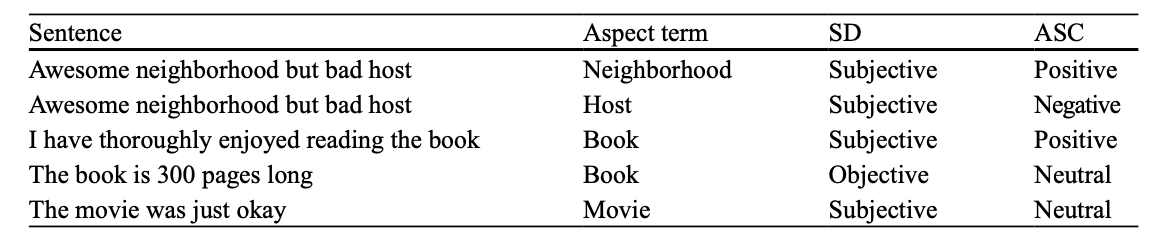
\includegraphics[width=1\linewidth]{img/SMABSA_sentence_examples.png}
    \caption{Input and Ouputut Notation for SMABSA}
\end{figure}

\subsubsection{General Architecture Overview}
The proposed Multitask Learning Approach is built upon a BERT Embeddings Layer, which shares results to 2 Bi-LSTM networks, one for each task. After both forward and backward contextual dependencies of tokens are captured, a self-attention mechanism follows to highlight the relevant words of input sequence for classification. The weighted results of the self-attention mechanism are fed into a Neural Tensor Network, which  captures the complex interactions between the task-specific representations and finally, its ouputs are passed in a classifcation mechanism for the final decisions to be extracted. You can see a generalized schema of the architecture in the image below, followed by a more specialised 
and analytical view on each of the framework's component.

\begin{figure}[h!]
    \centering
    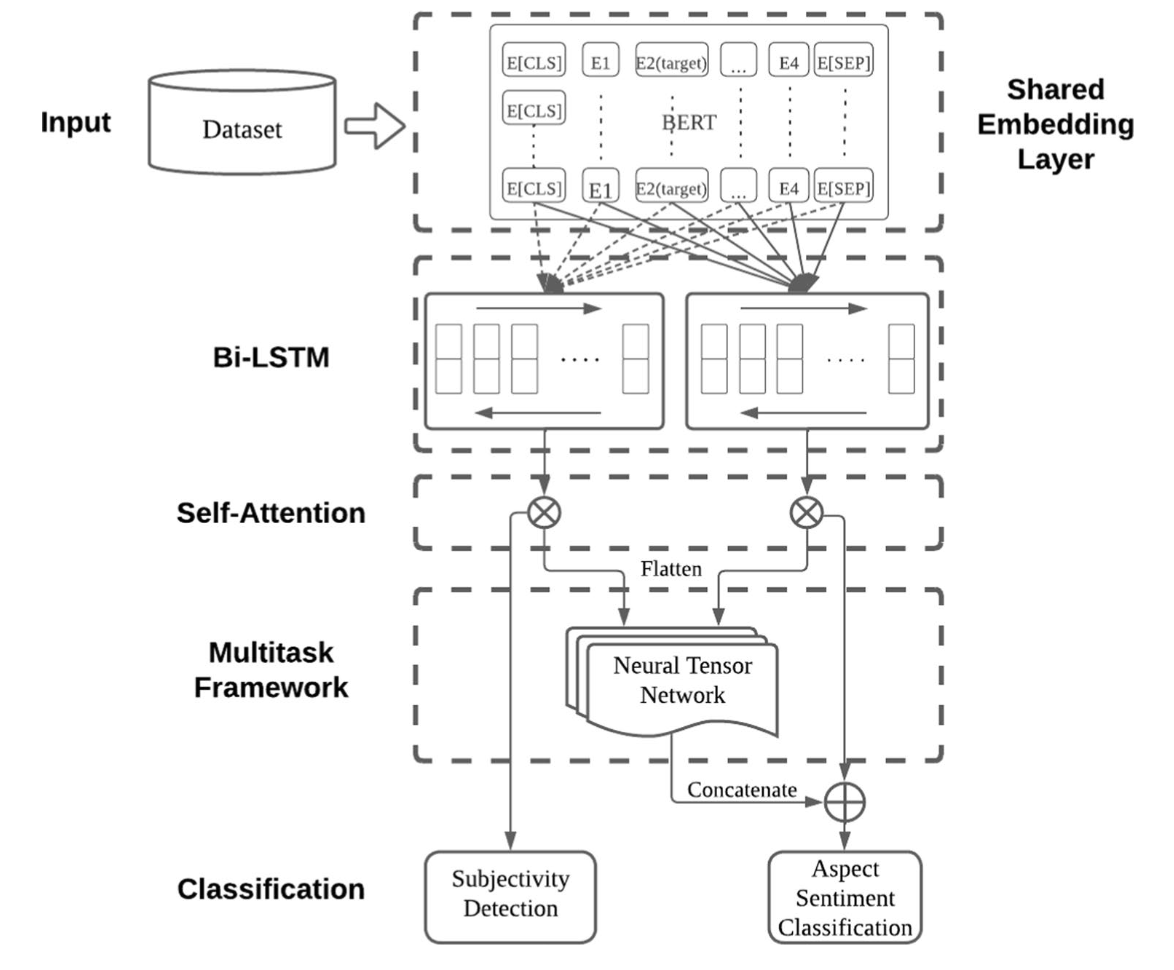
\includegraphics[scale=0.4]{img/SMABSA_architecture.png}
    \caption{Abstract Architecture Schema for SMABSA}
\end{figure}

\subsubsection{Shared Embedding Layer \& Bi-LSTM Networks}
The first step is the passing of our input, that is the sentence and aspect terms, into a shared embedding layer. The input is tokenized using WordPiece Tokenizer and then forwarded into the BERT Encoder. In that way, contextualized embeddings are generated for each token in the sequence. The output is a sequence of tokens ($H=\{h_0,h_1,...,h_n\}$), where $h_i$ is the hidden output of the BERT model in the i-th position. The BERT version used in this framework is BERT Base, which may not have the same number of parameters as BERT Large, it is much more computationally efficient. The BERT Encoder's Layers are fed into 2 Bi-Directional Long Short-Term Memory (LSTM) Modules, one for each task, which decompose H and learn the context-rich task-specific representations for the 2 subtasks. The following forward and backward contextual dependencies are enabled:
\begin{align}
h_t^{\text{forward}} &= \mathrm{LSTM}_{\text{forward}}(h_t, h_{t-1}^{\text{forward}}) \\
h_t^{\text{backward}} &= \mathrm{LSTM}_{\text{backward}}(h_t, h_{t+1}^{\text{backward}}) \\
h_t^{\text{BiLSTM}} &= \left[ h_t^{\text{forward}} \,;\, h_t^{\text{backward}} \right]
\end{align}

\subsubsection{Self Attention Layer}
To capture which words have the biggest impact on the classifcation of our sentence, a Self-Attention Layer is added. Having the embedding input H from the Shared Embedding Layer and Bi-LSTM Networks, we calculated weighted scores a ($a=\{a_0,a_1,...,a_n\}$) for each token, which represent the crucial meaning that it has on our 2-task classification. We mutliply a with H, so we get the weighted represenation for each input token.
\begin{align}
\alpha &= \mathrm{softmax}\left(W_b^{T} \cdot \tanh\left(W_a \cdot H\right)\right) \\
v &= \alpha \cdot H^{T}
\end{align}

\subsubsection{Neural Tensor Network (NTN)}
The weighted word representation obtained by the Self-Attention Layer is flattened before it is inputed in the Neural Tensor Network (NTN). NTN is the heart of multitask learning, as it captures the interactions between ABSA and SD and is able to develop the complex joint representations of both tasks in a single multitask framework. The combination of the 2 tasks happens with the help of a bilinear tensor transformation, which is defined by the following equation:
\begin{align}
v_{\text{NTN}} &= \tanh\left((v_{\text{subj}} \oplus v_{\text{asc}}) W + (v_{\text{subj}})^{T} \cdot G \cdot v_{\text{asc}} + b \right)
\end{align}

\subsubsection{Classification Layer}
The final component of the architecture is of course the classification part. There 2 classification layers, one for ASC and one for SD. More specifically:

\begin{itemize}
    \item \textbf{Subjectivity Detection (SD)}:The output of Self-Attention Layer as the represenation of the input sentence, which is later passed through a fully connected layer followed by softmax.
    \begin{align}
    \rho_{\text{subj}} &= \mathrm{softmax}\left(v_{\text{subj}} \cdot W_{\text{subj}} + b_{\text{subj}}\right) \\
    y_{\text{subj}} &= \arg\max\left(\rho_{\text{subj}}[j]\right)
    \end{align}
    The output is either 0 or 1, corresponding to objective or subjective.
    \item \textbf{Aspect Sentiment Classification (ASC)}:Concatenation of NTN Ouput with Self-Attention Output, again passed through fully connected layer with softmax activation.
    \begin{align}
    \rho_{\text{asc}} &= \mathrm{softmax}\left((v_{\text{asc}} \oplus v_{\text{NTN}}) \cdot W_{\text{asc}} + b_{\text{asc}}\right) \\
    y_{\text{asc}} &= \arg\max\left(\rho_{\text{asc}}[k]\right)
    \end{align}
    The ouput is 0, 1 or 2, corresponding to positive, negative or neutral.
\end{itemize}

\subsubsection{Training Objective}
For optimization, a loss-function that combines losses from both tasks was used. The \textbf{Categorical Cross-Entropy Loss Function} which is used as the objective function is:

\begin{align}
\mathcal{L}_{\text{ABSA,SD}} &= -\frac{1}{N} \sum_{i=1}^{N} \sum_{j=0}^{C-1} y_{ij}^{*} \log\left(P_i[j]\right)
\end{align}

The total loss is the aggregated sum of the loss of both tasks:

\begin{align}
\mathcal{L}_{\text{total}} &= \mathcal{L}_{\text{ABSA}} + \mathcal{L}_{\text{SD}}
\end{align}

\subsection{Ablation Study}
The Ablation Study, which is the validation of the contribution of each architectural component, offers very useful insight in the model's overall perfromance. Each component was removed one at a time and experiments
would be ran on each new subversion of the framework. The results on the corresponding paper show us that the entire hypothesis that this whole study was based on, which is that by assigning SD as an auxiliary subtask
the performance of the ABSA task will improve and therefore better results will be provided, turns out to be true. \textbf{The removal of the Subjectivity Detection component results to the decrease of both accuracy and F1-Score}.

\begin{table}[htpb]
\centering
\begin{tabular}{lll}
\toprule
Model variant & Accuracy (\%) & F1-score (\%) \\
\midrule
SMABSA (full model) & 88.15 & 87.26 \\
w/o Subjectivity detection (SD) & 83.92 & 69.81 \\
w/o Bi-LSTM & 86.45 & 85.53 \\
w/o Self-attention & 86.88 & 85.99 \\
w/o NTN (using concatenation) & 87.21 & 86.34 \\
\bottomrule
\end{tabular}
\caption{Ablation study results}
\label{tab:ablation_SMABSA}
\end{table}


\section{Domain-Adaptive PreTraining using transformer-based models for occupational safety applications}

\subsection{Introduction}
Even though occupational safety should have been addressed as soon as possible as state-of-the-art technologies have emerged, it remains a persistent global challenge. While on the past structured datasets were used to mine data related to this field, the main source of data should be taken from unstructured data, such as accident text-based reports, as they offer
a significant context source. Such sources can be valuable to train models that know how to extract the contextual meaning out of such documents, and one of the best frameworks that can be used today is \textbf{Bidirectional Encoder Representations for Transformers (BERT)}. This research focuses on adding another stage of pre-training on these models, a technique
called \textbf{Domain-Adaptive PreTraining (DAPT)} to give additional contextual boost to the already pre-trained BERT model. The experimental phase includes implementation on the BERT model itself, as well as a variant of it called \textbf{A Light BERT (ALBERT)}. A pipeline is created where each of these 2 models are used to process natural language and thus 2 new frameworks
occur, \textbf{safetyBERT} and \textbf{safetyALBERT}. After training on an extensive dataset of multiple sources, the results that are concluded
are optimal comparing to other contemporary frameworks and prove how DAPT enhances language understanding in domains such as occupational safety and hazards.

\subsection{Methodology Overview}
We are now going to see the consisting parts of the framework. Keep in mind the the central premise of the study is to show that pre-trained language models, like BERT and ALBERT which we use, can benefit by an additional layer of pre-training, that being DAPT, as it will increase the the model's comprehension of domain-specific nuances. The 3 parts of our framework are the following:

\begin{enumerate}
    \item \textbf{Multi-Source Domain Corpus Development}: Analyzes the creation of the DAPT training dataset, including data cleaning and pre-processing techniques.
    \item \textbf{Domain-Adapative PreTraining}: Pre-training BERT and ALBERT on the previously created dataset, to further increase the model's ability on handling safety occupation-based documents. 
    \item \textbf{Downstream Domain-Specific Fine-Tuning}: The fine tuning following the pre-training of the previous step to validate the model's ability on real life data and experimentally assess its abilities.
\end{enumerate}

A more analyzed view on the parts can be seen on the following image. On the rest of this analysis, we will furthermore develop the decisions and implementions on the framework's modules.

\begin{figure}[h!]
    \centering
    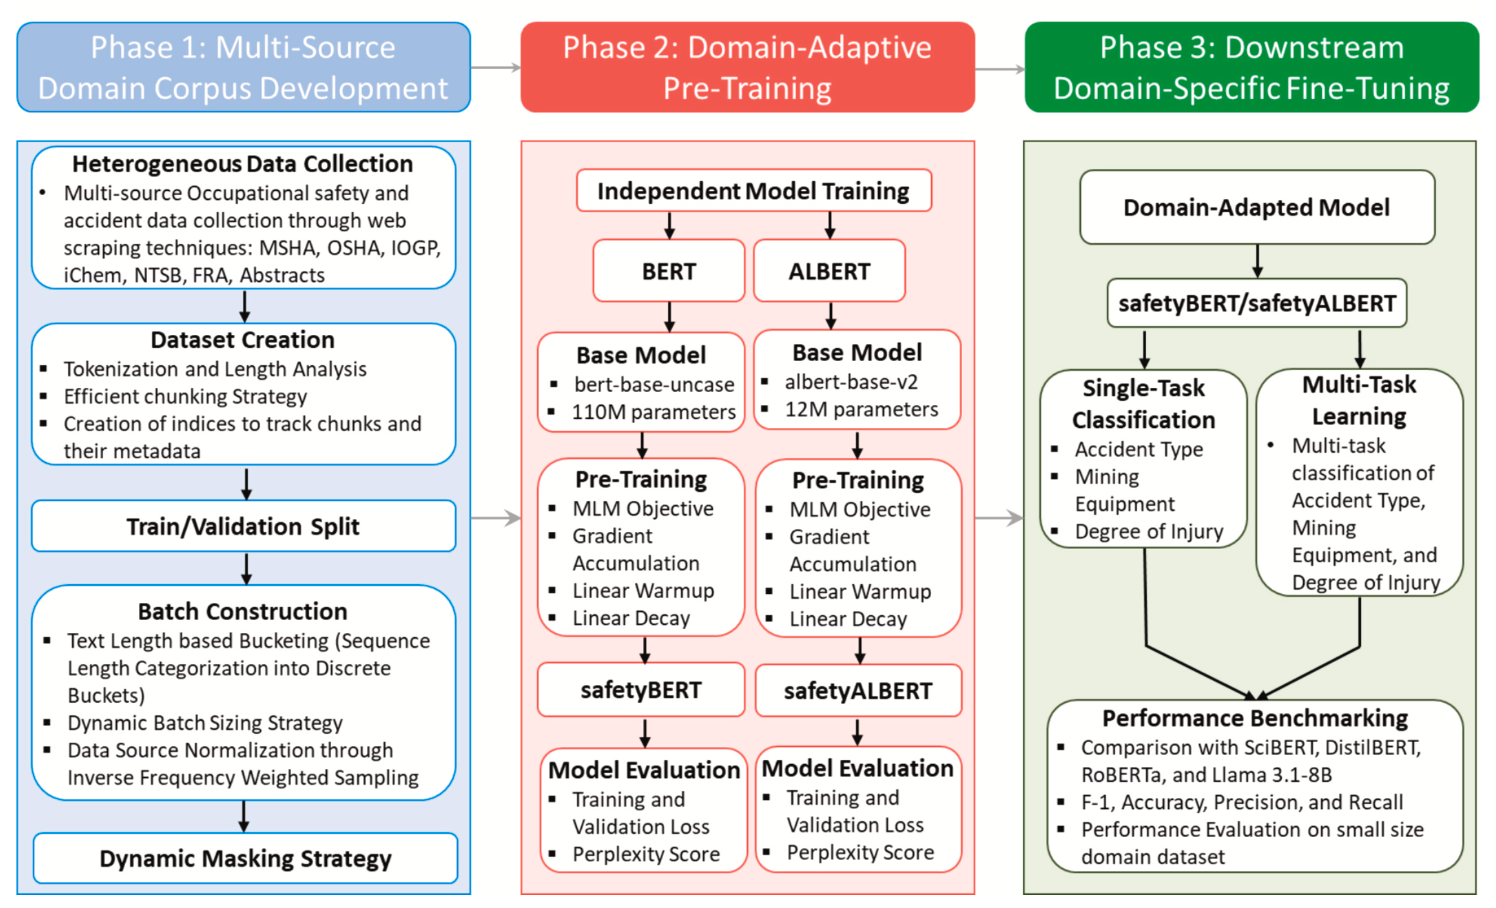
\includegraphics[scale=0.6]{img/DAPT_framework.png}
    \caption{Framework Overview}
\end{figure}

\subsection{Multi-Source Domain Corpus Development}
What kind of dataset is needed to enhance the already pre-trained language models and make them more task-specified on the specific domain of industrial hazards? The structured dataset consists of multiple sources of corpus, so rich as to satisfy the levels of the required terminology and contextual meaning of the field.

\subsubsection{Sources}
The new datasets consists of 7 sources across academic literature, regulatory agencies and industrial organizations, where signifcant data were extracted using 2 frameworks, the Academic Abstract Collection Framework and Accident Narrative Collection Framework. Moreover, academic journal abstracts from well-known publishers were also incorporated, to broaden the model's terminology. Finally, 
more unstructured data sources were, such as incident narratives, were also collected from multiple regulatory and incident sources. The resulting corpus seems perfectly balanced in technical terminology and practical language, ensuring that the included language patterns will effectively boosts the model's comprehension on the targeted domain.

\subsubsection{Tokenization}
In order for our language models to process the newly created corpus, we need to prepare our data for efficient training. The 2 steps we are following are tokenization and input sequence processing. Tokenization is a pre-processing technique, which breaks the input into smaller parts called tokens, which will be the input to our language models. For \textbf{BERT} we are using the pre-trained \textbf{WordPiece} Tokenizer
and for \textbf{ALBERT} we are using the \textbf{SentencePiece} Tokenizer. Also, special tokens, such as [CLS] for Classification or [MASK] for masking tokens, were added according to the requirements of the MLMs.

\subsubsection{Sequence processing and Categorization for batch construction}
Another problem that needs to be faced is variable input length, as the self-attention operation used in transformer-based models seems to not scale on an efficient rate. This problem is present in our newly created corpus, which seems to be highly heterogenous in the matter of length. An upper token limit set to 512 was set to for our standard width context window size in BERT and ALBERT and for texts exceeding this limit, 
overlapping chunking strategy was implemented with a predefined stride parameter. Last but not least, for computational efficiency, the sequences were categorized in diferrent buckets/batches, according to the token length. Inside each bucket, all the tokens were padded to the length of the longest sequence, saving both memory and facing the variable lenght input problem. Before training, the batches are randomly shuffled to ensure diversity,
keeping in the same times the efficient memory management.

\subsubsection{Source Domain Imbalance}
The last challenge that arises in our data collecting and pre-processing phase is the source imbalance in the newly created corpus. This is unwanted, as it can bias the model towards one end and thus overfit. To face this, the authors introduce a weighted sampling approach, to fairly sample sources during batch construction. The equation used for the weights is the following:

\begin{align}
\omega_s = \frac{N_{\text{total}}}{N_s}
\end{align}

where $\omega_s$ is the weight for source $s$, $N_{\text{total}}$ is the total number of samples and $N_s$ is the number of samples from source $s$. From source $s$, we sample with a probability of:

\begin{align}
P(x_i) \propto \omega_{s(i)}
\end{align}

This approach ensures that when random shuffling the batches before training, all sources get the same chance of being chosen and thus we have the same occurence from sequences across all sources.

\subsection{Domain-Adapative PreTraining}
As previously metioned, this study takes already pre-trained language models, which are BERT and ALBERT, and 'force' them in another round of pre-training on a specific field to specify the model's fit to it. This procedure, also known as \textbf{Domain-Adapative PreTraining (DAPT)}, is believed to improve results in downstream tasks, such as increased contextuality on the new field. In this section, 2 basic topics of DAPT are analyzed: \textbf{MLM} and \textbf{Domain-Adapated Model Evaluation}.

\subsubsection{Masked Language Modeling (MLM)}
Even though it was first suggested that the pre-training of BERT models should consist of 2 parts, masking and Next Sentence Prediction (NSP), only masking is used in this study due to the proven inefficiency of NSP. There are 5 stages in which the BERT and ALBERT models go thorugh DAPT:

\begin{enumerate}
    \item \textbf{Data Preparation}: As analyzed in the previous section.
    \item \textbf{Input Embedding Construction}: The Input Embeddings are an aggregation of \textbf{Token Embeddings}, \textbf{Segment Embeddings} and \textbf{Position Embeddings}, where BERT uses full-dimensional embeddings (768 dimensions) and ALBERT uses a factorized approach with less parameters (128 dimensions), projected to the original 768 dimensions.
    \item \textbf{Input Masking}: Tokens are strategically and dynamically replaced with [MASK] special tokens, where the model tries to predict them. 
    \item \textbf{Masked Sequence Processing}: The masked sequence are processed through the transformer encoded architectures, where BERT uses independent parameters across 12 layers and ALBERT employs parameter sharing, thus reducing once again the number of them.
    \item \textbf{MLM Prediction}: The predictions after masking are finally made, using an FFNN and the softmax activvation function. 
\end{enumerate}

For optimization, the following cross-entropy loss function is applied:

\begin{align}
L_{\text{MLM}} = - \sum \log P(w_i \mid \tilde{w})
\end{align}

 , where $w_i$ is the correct token at masked position i and $\tilde{w}$ is sequence with masked tokens. The function is minimized using the AdamW optimizer with weight decay and learning rate.

\subsubsection{Domain-Adapted Model Evaluation}
In this study, both Intrinsic and Extrinsic Model Evaluation Metrics are used. For \textbf{Intrinsic Evaluation}, Pseudo-Perplexity is a meaningful metric for BERT evaluation. Let $W=(w_1,w_2,...,w_n)$ be a sequence of tokens. The \textbf{pseudo-log-likelihood (PLL)} is defined as:

\begin{align}
\text{PLL}(W) = \sum_{t=1}^{|W|} \log P(w_t \mid W_{\setminus t}; \theta)
\end{align}

, where $W_{\setminus t}$ are all the tokens in the sequence except the tokens in position t. \textbf{PPPL} is derived from this as a normalization over sequence length:

\begin{align}
\text{PPPL}(W) = \exp\left( -\frac{1}{N} \cdot \text{PLL}(W) \right)
\end{align}

Finally, for fair comparison between models with different subword tokenization schemes, like BERT and ALBERT are, a word-normalized version is used:

\begin{align}
\text{PPPL}_w(W) = \exp\left( -\frac{1}{N_w} \cdot \text{PLL}(W) \right)
\end{align}

For \textbf{Extrinsic Evaluation}, as task-specific classification will be added in the fine-tuning section, we use the \textbf{Weighted F1 Score}, as it effectively balances the precision-recall trade off.

\subsection{Downstream Domain-Specific Fine-Tuning}
Now that the language models have passed another phase of pre-training, the domain-adapted one, it is time to evaluate that procedure on downstream domain-specific classification tasks. The evaluation happens by mainly comparing the models before and after DAPT and against other diverse baseline models. The fine-tuning phase consists of the \textbf{Corpus Development},
\textbf{Data Preprocessing} and finally we will see some \textbf{Fine-Tuning Approaches}.

\subsubsection{Corpus Development}
The first step is the development of a specialized corpus to fine-tune the 2-time pre-trained language models. This corpus consists of unstructured data from the MSHA Accident Narratives, from the period of January 2022 to February 2025. We tested it on classification of accident type, mining equipment and degree of injury, using both single task and multi task learning approaches. To test the models on smaller sources, the Alaska mining injuries insurance claim was employed, which was fine-tuned on claim type and injured body part classification.

\subsubsection{Data Preprocessing}
The MSHA Dataset initially contains 40 classes for accident type and 75 classes for mining equipment. In order to enable a more generalized learning for the model, the authors group these categories and end up in a reduced number of more meaningful categories, 9 for accident type and 8 for mining equipment. To increase data quality, authors also remove entries with missing values. For the Alaska mining accident insurance claim for the non-fatal accident dataset, only missing values were removed again to ensure the quality of data.

\subsubsection{Fine-Tuning Approaches}
Next, some fine-tuning strategies will be presented to show how DAPT can further be optimized. Firstly, \textbf{Single-Task Learning} is when each classification objective is addressed independently. As previously stated, safetBERT and safetyALBERT are utilized and a simple classification layer is added. Big importance must be given to the final hidden state of the classification layer, which carries the special token [CLS]. During single-task classification fine-tuning, all parameters remain frozen and the quality of classification is calculated with Cross-Entropy Loss. Secondly, on the same fashion, \textbf{Multi-Task Learning}
trains multiple classification objectives at the same times. This can be helpful, as tasks can develop inherent relationships between them and thus a more reliable result is given. The implementation utilizes a shared transformer encoder and ReLU as activation function. Again, all parameters remain frozen during training and Loss Balancing is the weighted sum of the individual task losses, with equal weights so no task is favored over another. Lastly, \textbf{Hyperparameter Optimization} is of important significance to the model's efficiency as well. The authors use grid search with n-fold cross-validation to identify optimal model 
configurations for both single-task and multi-task learning frameworks, with more evaluation metrics such as F1-Score, Precision, Recall, etc. used to find the optimal hyperparameters.

\clearpage
\section{Extended Literature Review}

\subsection{Representation Learning: Matryoshka Representation Learning}

A implicit assumption underlying most embedding-based systems is that all downstream 
tasks require the same representational capacity. In practice, however, a coarse 
document retrieval task and a fine-grained semantic similarity task have fundamentally 
different precision requirements, yet both are typically served by the same 
fixed-dimensional embedding vector. This rigidity forces practitioners into an 
uncomfortable tradeoff: train a large, expensive embedding model for maximum accuracy, 
or train a smaller, faster one and accept a performance penalty. \citet{kusupati2022matryoshka} 
address this limitation directly with \textit{Matryoshka Representation Learning} (MRL).

The core insight of MRL is deceptively simple: rather than optimizing a model to 
produce a single fixed-size embedding, train it such that the first $m$ dimensions 
of the output vector are independently meaningful for every $m$ in a chosen set 
$\mathcal{M} = \{8, 16, 32, 64, \ldots, d\}$. This is achieved by modifying the 
training loss to be a weighted sum of losses computed at each target dimensionality:

\begin{equation}
    \min_{\{\mathbf{W}^{(m)}\}_{m \in \mathcal{M}},\, \theta_F} 
    \frac{1}{N} \sum_{i \in [N]} \sum_{m \in \mathcal{M}} 
    c_m \cdot \mathcal{L}\!\left(\mathbf{W}^{(m)} \cdot F(x_i; \theta_F)_{1:m};\, y_i\right)
\end{equation}

where $c_m$ is a scalar weight controlling the relative importance of each 
dimensionality during training, $\mathbf{W}^{(m)}$ is a learned linear layer 
that projects the first $m$ dimensions of the embedding into the classification 
space, and $\mathcal{L}$ is the multi-class softmax cross-entropy loss computed 
against the ground truth label $y_i$. The rest of the training pipeline remains 
unchanged, MRL is a modification of the loss function, not the architecture.

The authors also propose \textit{MRL-E} (Efficient MRL), which eliminates the need 
for separate linear projection layers per dimensionality. Instead of projecting the 
full representation down to $m$ dimensions via learned weight matrices $W_m$, MRL-E 
simply truncates the embedding vector at position $m$ directly. This means the 
overhead of MRL-E over standard embedding training is negligible, as no additional 
parameters or projection steps are introduced.

The key empirical finding is that MRL embeddings, when truncated to $m$ dimensions, 
achieve approximately 97--99\% of the performance of a dedicated model independently 
trained at that same dimensionality $m$. Critically, this holds across a single 
model, meaning one MRL-trained model can replace an entire family of fixed-size 
embedding models without retraining. This was validated across large-scale 
classification and retrieval benchmarks, where lower-dimensional MRL embeddings 
matched the accuracy of their dedicated counterparts while offering substantial 
reductions in inference latency and memory footprint.

The authors draw an analogy to the brain's natural coarse-to-fine processing 
hierarchy, where rough semantic distinctions are established before fine-grained 
details are resolved. MRL operationalizes this principle in the embedding space: the 
early dimensions capture the most salient semantic structure, with subsequent 
dimensions progressively refining the representation. Notably, this property 
generalizes to intermediate dimensionalities not explicitly included in $\mathcal{M}$ 
during training, suggesting that the learned representations are smoothly structured 
rather than discretely partitioned.

The relevance of MRL to the broader themes of this report is direct. RexBERT's 
evaluation on retrieval benchmarks such as ESCI implicitly relies on the assumption 
that embedding dimensionality is fixed at inference time. MRL challenges this 
assumption, offering a principled framework for adaptive-precision retrieval that 
could be applied on top of any encoder, including the domain-specialized encoders 
explored in this report.

\subsection{Catastrophic Forgetting in Large Language Models}

Catastrophic forgetting refers to the tendency of neural networks to lose previously
acquired capabilities when fine-tuned on new tasks sequentially, without access to
prior training data. While this phenomenon has been documented empirically across
many model families, the internal mechanisms driving it in large transformer-based
models remained poorly understood. \citet{imanov2026mechanistic} address this gap
with a systematic mechanistic analysis of catastrophic forgetting during sequential
fine-tuning, studying six contemporary LLM architectures spanning 109B to 1.5T
parameters across twelve task sequences of varying inter-task similarity.

The study identifies three primary mechanisms that collectively drive forgetting,
each operating at a distinct architectural level and timescale.

\textbf{Attention Mechanism Disruption.} The first and earliest mechanism involves
the disruption of attention heads in the lower layers of the network. When these attention weights were frozen during fine-tuning, forgetting was reduced by 64 percent compared to full fine-tuning, establishing attention mechanisms as the primary driver of
early-stage forgetting. Approximately 15 to 23 percent of attention heads across all
layers underwent severe reorganization, defined as weight changes exceeding 2.5
standard deviations from the mean. Critically, of these severely disrupted heads,
only 31 percent showed high activation levels when processing new task data, indicating
that fine-tuning is largely non-selective, disrupting many heads that play no role
in acquiring the new capability. This was confirmed causally by an ablation
experiment: restoring the 20 percent most disrupted heads to their pre-fine-tuning
state recovered 47 percent of lost performance on the original task while degrading
new task performance by only 8 percent. The asymmetry of this result confirms that
the fine-tuning process overwrites task-irrelevant attention circuits as collateral
damage rather than targeting specific parameters.

\textbf{Representational Drift in Intermediate Layers.} The second mechanism
operates at the level of hidden representations in the intermediate layers of the
model. Using Centered Kernel Alignment (CKA), a metric measuring representational
similarity before and after fine-tuning, the authors found that intermediate layers
(layers 8 to 16 in 24-layer architectures) exhibited the largest drift, with CKA
scores decreasing by 0.32 to 0.47 on a 0 to 1 scale. Principal component analysis
revealed that the leading components, accounting for 60 to 75 percent of
representational variance, rotated by 35 to 52 degrees on average during fine-tuning,
while higher-order components remained relatively stable. This suggests fine-tuning
preferentially disrupts the dominant, most general representational structure of the
model rather than its more granular, task-specific features. Notably, drift magnitude
showed no significant correlation with task-relevance of individual dimensions
(Pearson $r = 0.12$, $p = 0.24$), confirming that representational drift is
indiscriminate. A realignment intervention that restored intermediate representations
to their pre-fine-tuning geometry recovered 38 percent of lost task performance with
only 6 percent degradation on the new task.

\textbf{Gradient Interference.} The third mechanism concerns the optimization
dynamics during sequential fine-tuning. For any two tasks, one can compute the
cosine similarity between their respective gradient vectors in parameter space, that
is, the degree to which the two tasks pull the model's parameters in compatible or
conflicting directions. The authors find that when gradient cosine similarity falls
below $-0.3$, indicating substantial conflict, forgetting rates increase by 2.4 times
compared to conditions of positive gradient alignment. Interference localized
disproportionately to the query and key projection matrices of the attention layers,
with 67 percent of these parameters experiencing gradient conflicts, compared to
34 percent for value projections and 29 percent for feedforward weights. Importantly,
gradient alignment measured during the very first epoch of fine-tuning, before any
observable accuracy degradation, already predicted final forgetting magnitude with
$r = -0.79$ ($p < 0.001$), establishing gradient interference as a practical early
warning signal for catastrophic forgetting.

\textbf{Loss Landscape Flattening.} The fourth mechanism operates at the level of
loss landscape geometry. After training on a task, the model resides in a sharp
minimum in parameter space, characterized by high curvature and a strong restoring
force that would pull the model back toward good performance if it drifts. Sequential
fine-tuning progressively flattens this minimum: the maximum Hessian eigenvalue for
the original task's loss function decreased from 147.3 at convergence to 34.2 after
three subsequent tasks. As the landscape flattens, the restoring force disappears
and forgetting becomes increasingly irreversible. Critically, this flattening was
detectable 1 to 2 epochs before any observable accuracy drop, making it another
prospective signature of impending forgetting.

\textbf{Integrated Model and Implications.} These four mechanisms interact
synergistically across different timescales. Gradient interference and attention
disruption dominate in early epochs (1 to 2), representational drift accumulates
progressively over epochs 3 to 5, and loss landscape flattening emerges as a
longer-term consequence after epoch 4 or more. A combined intervention targeting
both attention head restoration and representational realignment recovered 71 percent
of original task performance, demonstrating that the mechanisms are partially
independent and their effects additive.

One counterintuitive finding is that higher inter-task similarity was associated with
more severe forgetting in these experiments, not less. The authors attribute this to
the fact that similar tasks produce gradients that appear globally aligned but
introduce subtle, localized conflicts in specific parameter subsets, particularly the
query and key projection matrices, creating a false impression of compatibility while
damage accumulates in specific circuits.

For the broader context of this report, these findings carry direct implications.
All four assigned papers involve some form of continued pre-training or fine-tuning
of BERT-based encoders, and the design choices made in each, such as RexBERT's
phased training curriculum, safetyBERT's weighted corpus sampling, and TSAPM-BERT's
selective layer freezing, can be understood as implicit mitigations of the mechanisms
identified here. It is worth noting, however, that the paper's experimental scope
is limited to decoder-only and mixture-of-experts architectures. Whether the same
three mechanisms govern forgetting in encoder-only models like BERT remains an open
question, and extending this mechanistic framework to encoders represents a natural
direction for future work.

\subsection{Mixture of Experts Approaches in Dense Retrieval Tasks}
As it is known, the primary goal of Information Retrieval is to efficiently identify, rank and deliver the most relevant information from a large collection of data in response to a user's query. In the past, Sparse Retrieval Models (sparse-lexicon models) were used as a solution to IR's goal. Even though the keyword matching technique that SRMs supported between the user's query and the document
made sense at first, its big gap was that such models were missing the semantic similarity between words or phrases. For example, if a user would search for 'fast electric car' documents including exactly these words would be returned. However, documents containing informations about 'speedy EV', which semantically refer to the same topic as the user's query, would be missed. For that reason, Dense Retrieval
Models (DRMs) were proposed. DRMs are based on the Transformer model, and more specifically on BERT, therefore allowing the networks to capture semantic meaning between query and document. DRMs map both queries and documents into the embedding space, where semantic similarity equals to geometric closeness and for that reason a similarity score is finally employed to assess the resemblance between query and document.
A big problem that DRMs faced was generalization, as they perform really well on specific tasks they are fine tuned to but lack the ability of generalizing on larger domains. The authors propose a framework by employing a single block Mixrure-of-Experts (SB-MoE) right after the final Transformer layer of the underlying DRMs. 

\subsubsection{Mixture-of-Experts Block}
The SB-MoE added after the DRMs consists of multiple pairs of Feed-Forward Networks (FFNs), where each one is specialized in something different than the others (that's why they are called 'experts'). After an input, a gating function (neural network which assigns a weight to each expert) determines how relevant each expert is to the input and along a pooling strategy, the final prediction of the model.

\subsubsection{Architecture}
SB-MOE builds on a standard bi-encoder architecture, where one of four underlying base models — Contriever (110M parameters), BERT-Base (110M), BERT-Small (29M), or TinyBERT (14.5M) — independently encodes the query and document into dense vector embeddings. 
The SB-MoE is then appended after the final Transformer layer of whichever base model is used, acting on both the query and document embeddings simultaneously . The gating function, consisting of a single hidden layer that halves the vector dimension followed by an output layer
sized to the number of experts, is trained end-to-end in an unsupervised manner alongside the underlying DRM and the experts themselves. Each expert follows the adapter architecture, with a down-projection layer that halves the input dimension and an up-projection that restores it, plus a skip connection for residual learning. At inference time, the model operates in one of two modes:
$SB-MOE_{TOP-1}$, which selects only the expert assigned the highest gating score, or $SB-MOE_{ALL}$, which produces a weighted sum across all experts. The final enriched embeddings from either variant are then compared via dot product to compute query-document relevance scores. The authors look to answer in the 3 following Research Questions (RQs) to evaluate their framework:

\begin{itemize}
    \item{\textbf{RQ1}}: How does SB-MOE compare, in terms of retrieval effectiveness, to the fine-tuned version of the underlying DRM? - The authors fine-tune each DRM as baseline experiments to compare to their model including SB-MoE (\textbf{\texttt{FINE-TUNED}}).
    \item{\textbf{RQ2}}: To what extend can the observed performance gains be attributed to the learned gating function and to the experts’ ability to capture useful textual characteristics? - The authors employ enother baseline where they assign random weights to the gating function (\textbf{\texttt{RANDOM-GATE}}). 
    \item{\textbf{RQ3}}: Can SB-MOE generalize well across multiple domains and tasks without additional fine-tuning? - The authors fine-tune all 4 DRMs on the MSMARCO dataset, which is widely adopted for zero-shot evaluation.
\end{itemize}

\begin{figure}[h!]
    \centering
    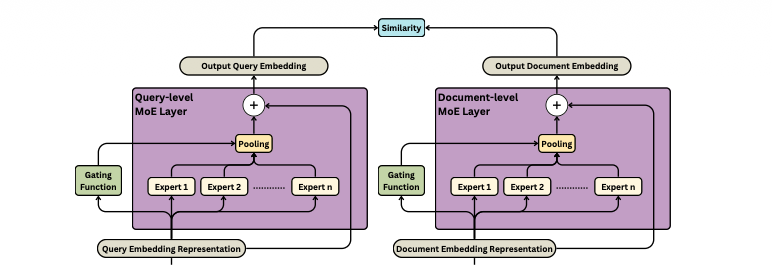
\includegraphics[width=1\linewidth]{img/SB_MoE_Architecture.png}
    \caption{SB-MoE Architecture Overview}
\end{figure}

\subsubsection{Results}
The results demonstrate that SB-MOE delivers its most consistent and meaningful performance when integrated with lightweight base models, TinyBERT and BERT-Small, where it outperforms standard fine-tuning across both in-domain benchmarks and zero-shot evaluation on BEIR datasets. For larger models 
like BERT-Base and Contriever, the benefits are considerably less obvious, suggesting that models already rich in parameters leave little room for the additional expert layers to contribute meaningfully. Regarding the number of experts, the hyperparameter analysis reveals that no single configuration consistently dominates across all datasets
and metrics — while 6 experts was the default used throughout the main experiments, configurations with as few as 3 experts often performed competitively, and increasing beyond 6 did not reliably yield further gains. Finally, an extra analysis on the number of experts activated was performed. Despite configuring the model with up to 12 experts, only a subset of them — never more than 7 — were actually activated during inference 
across any collection. Notably, the 3-expert configuration achieves 100\% activation across all evaluated corpora, suggesting that a compact expert pool can be both fully utilized and effective, making SB-MOE an appealing choice for resource-constrained settings where efficiency is as important as retrieval performance.

\subsection{Multitask Learning for Sentiment and Emotion Analysis using resource constrained MobileBERT and DistilBERT}

As emotional recognition and sentiment analysis are emerging trend in the field of Natural Language Processing (NLP), and especially the task of calssifying both of them in a sentence (very crucial in the contemporary age for multiple tasks such as social media monitoring), the authors of this paper propose a refined framework that balances both high scores in metrics and low computational requirements.
To achieve that, lightweight transformers were used. The two kinds of lightweight transformers are (i) \textbf{Mobile Bidirectional Encoder Representations from Transformers (MobileBERT)} and (ii) \textbf{Distilled BERT (DistilBERT)}. Even though traditional methods to classify emotion recognition and sentiment analysis focus on single-task learning approaches, the authors adopt the idea of \textbf{multi-task learning} (training both tasks jointly), 
due to the fact that both tasks are closely related. In that manner, the sharing of overlapping features, contexts and semantic nuances allows the entire pipeline to perform better than it would have if we have focused on single-task learning. Let's dive deeper in the architecture of the pipeline.

\subsubsection{Pipeline Architecture}
The pipeline's architecture follows some finite steps that allows the model to perform emotional recognition and sentiment analysis using lightweight NLP models. These steps are:

\begin{itemize}
    \item{\textbf{Text Input}}: We begin with sampling the data that are going to be used for input in our framework.
    \item {\textbf{Data Augmentation}}: Data Augmentation is applied through random word deletion to introduce variability into training data, therefore enhancing model generalization and robustness.
    \item {\textbf{Lightweight Transformer Models}}: The next step focuses on our data being passed through MobileBERT and DistilBERT. Both models have a tradeoff between hitting high metric scores and parameter number. As we are going to discuss in the results section below, DistilBERT supposedly has better results compared to MobileBERT due to higher paramemter count and therefore higher computational intensity and MobileBERT hits more modest results, 
        but with much higher efficiency on realtime inference, which makes it more suitable for deployment as an edge device (e.g. mobile phone).
    \item{\textbf{Prototypical Networks}}: Protoypical Networks are used for metric-based classification for few-shot tasks. They work by computing a center for each class in the embedding space and when it is time to classify an item, in our case an utterance, the euclidean distance between the utterance and the prototypes center is being computed. Of course, the class with the smaller distance is selected for prediction. This approach is robust for class-imbalanced datasets as
        prototypes adapt dynamically to the class distribution and ensure discriminative embeddings. The formula used to compute Protoypical Network loss is $L_{\mathrm{proto}} = \frac{1}{N} \sum_{i=1}^{N} d\!\left(f(x_i), \mu_{y_i}\right)$ and it ensures the tight clustering of the utterance embeddings around around the class prototypes.
    \item{\textbf{Focal Weighted Loss Function}}: In another attempt to mitigate the class imbalance in the dataset, the focal weighted loss function is introduced. It introduces a modulating factor that adjusts depending on the difficulty of prediction for each class. It is computed using the formula $FL(p_t) = -\alpha_t (1 - p_t)^{\gamma} \log(p_t)$, where $p_t$ is the model's predicted probability for the correct class, $a_t$ is a weight assigned to a class t depending on the class' difficulty to be predicted
        and γ is a modulating factor, so the model will learn to focus on more difficult-to-classify examples. The final loss function is a weighted combination od focal weighted loss and protoypical network loss functions for both tasks.
    \item{\textbf{Shared Layers and Task-Specific Layers}}: Last but not least, the pipeline employs shared layers for leveraging common patters and detecting shared relation between the 2 tasks and task-specific layers for each task specifically. The former consists of transformer layers from our lightweight transformer models, while the latter of fully connected layers. Finally, Multi-Head attention is used to help the model focus better on emotinally-heavy part of a sentence, while cross-attention helps enabling
        the interaction between the two tasks.
\end{itemize}

\subsubsection{Results and Ablation Study}
The proposed framework achieved strong results on both benchmark datasets (MELD and IEMOCAP).The proposed framework achieved strong results on both benchmark datasets. DistilBERT reached 81\% weighted F1 for emotion and 77\% for sentiment on MELD, and 77\%/79\% on IEMOCAP. MobileBERT scored lower overall but remained competitive given its much smaller footprint, making it the better fit for truly resource-constrained deployments.
The ablation study broke down how much each component contributed. Removing the prototypical networks caused the steepest performance drop — 15 to 18 percentage points — confirming they're the backbone of the approach, particularly for handling imbalanced classes. Dropping the focal weighted loss cost around 4–5 points, showing it plays a meaningful but secondary role in pushing the model to focus on harder, minority-class examples. 
Data augmentation via random word deletion had the smallest impact, trimming only about 3 points when removed, though it still provided consistent gains across the board. The takeaway is clear: all three components work together, but the prototypical network is by far the most critical piece.

\clearpage
% --- BIBLIOGRAPHY SECTION ---
\bibliographystyle{plainnat}
\bibliography{citations/references}

\end{document}